\chapter{Results and Discussion}

This chapter synthesises the comprehensive analysis of the CTU-IoT-Malware dataset, the performance of various machine learning and deep learning models, and an in‐depth discussion of the implications for malware detection. The findings highlight how carefully engineered network flow features can be used to robustly discriminate between malicious and benign traffic, even in the absence of deep packet inspection.

\section{Dataset Characteristics and Exploratory Data Analysis}

\subsection{Dataset Overview}

The CTU-IoT-Malware dataset comprises 1,008,748 network connections, with a relatively balanced distribution of 53.5\% malicious and 46.5\% benign traffic. Table~\ref{tab:dataset_summary} summarises the key statistics, including the proportions of TCP (57.8\%), UDP (40.5\%), and ICMP (1.7\%) connections.

\begin{table}[htb]
\center
\begin{tabular}{lrr}
\hline
\textbf{Characteristic} & \textbf{Count} & \textbf{Percentage} \\
\hline
Total connections        & 1,008,748      & 100\%   \\
Malicious connections    & 539,473        & 53.5\%  \\
Benign connections       & 469,275        & 46.5\%  \\
\hline
TCP connections          & 583,134        & 57.8\%  \\
UDP connections          & 408,193        & 40.5\%  \\
ICMP connections         & 17,421         & 1.7\%   \\
\hline
\end{tabular}
\caption{Summary statistics of the analysed network traffic dataset.}
\label{tab:dataset_summary}
\end{table}

Further analysis revealed several important dataset characteristics:
\begin{itemize}
    \item \textbf{Class distribution}: A balanced proportion of malicious and benign traffic facilitates reliable model training.
    \item \textbf{Missing values}: Critical features such as \texttt{duration}, \texttt{orig\_bytes}, and \texttt{resp\_bytes} were missing in about 79\% of connections, necessitating careful preprocessing.
    \item \textbf{Attack diversity}: The vast majority (99.9\%) of malicious traffic in this dataset represents port scanning activities, a common precursor to more sophisticated attacks.
\end{itemize}

\subsection{Exploratory Data Analysis}

An extensive exploratory analysis was performed to reveal underlying patterns in the network traffic. Key insights include:

\paragraph{Protocol Analysis:}  
Figure~\ref{fig:protocol_distribution} shows that TCP is the predominant protocol. However, when disaggregated by traffic type (see Figure~\ref{fig:protocol_by_label}), TCP appears in 72.4\% of malicious traffic compared with only 40.9\% of benign traffic. In contrast, UDP is more common in benign traffic (46.2\%) and ICMP is almost exclusively used for network diagnostics in benign connections.

\begin{figure}[htbp]
    \centering
    \begin{subfigure}[b]{0.48\textwidth}
        \centering
        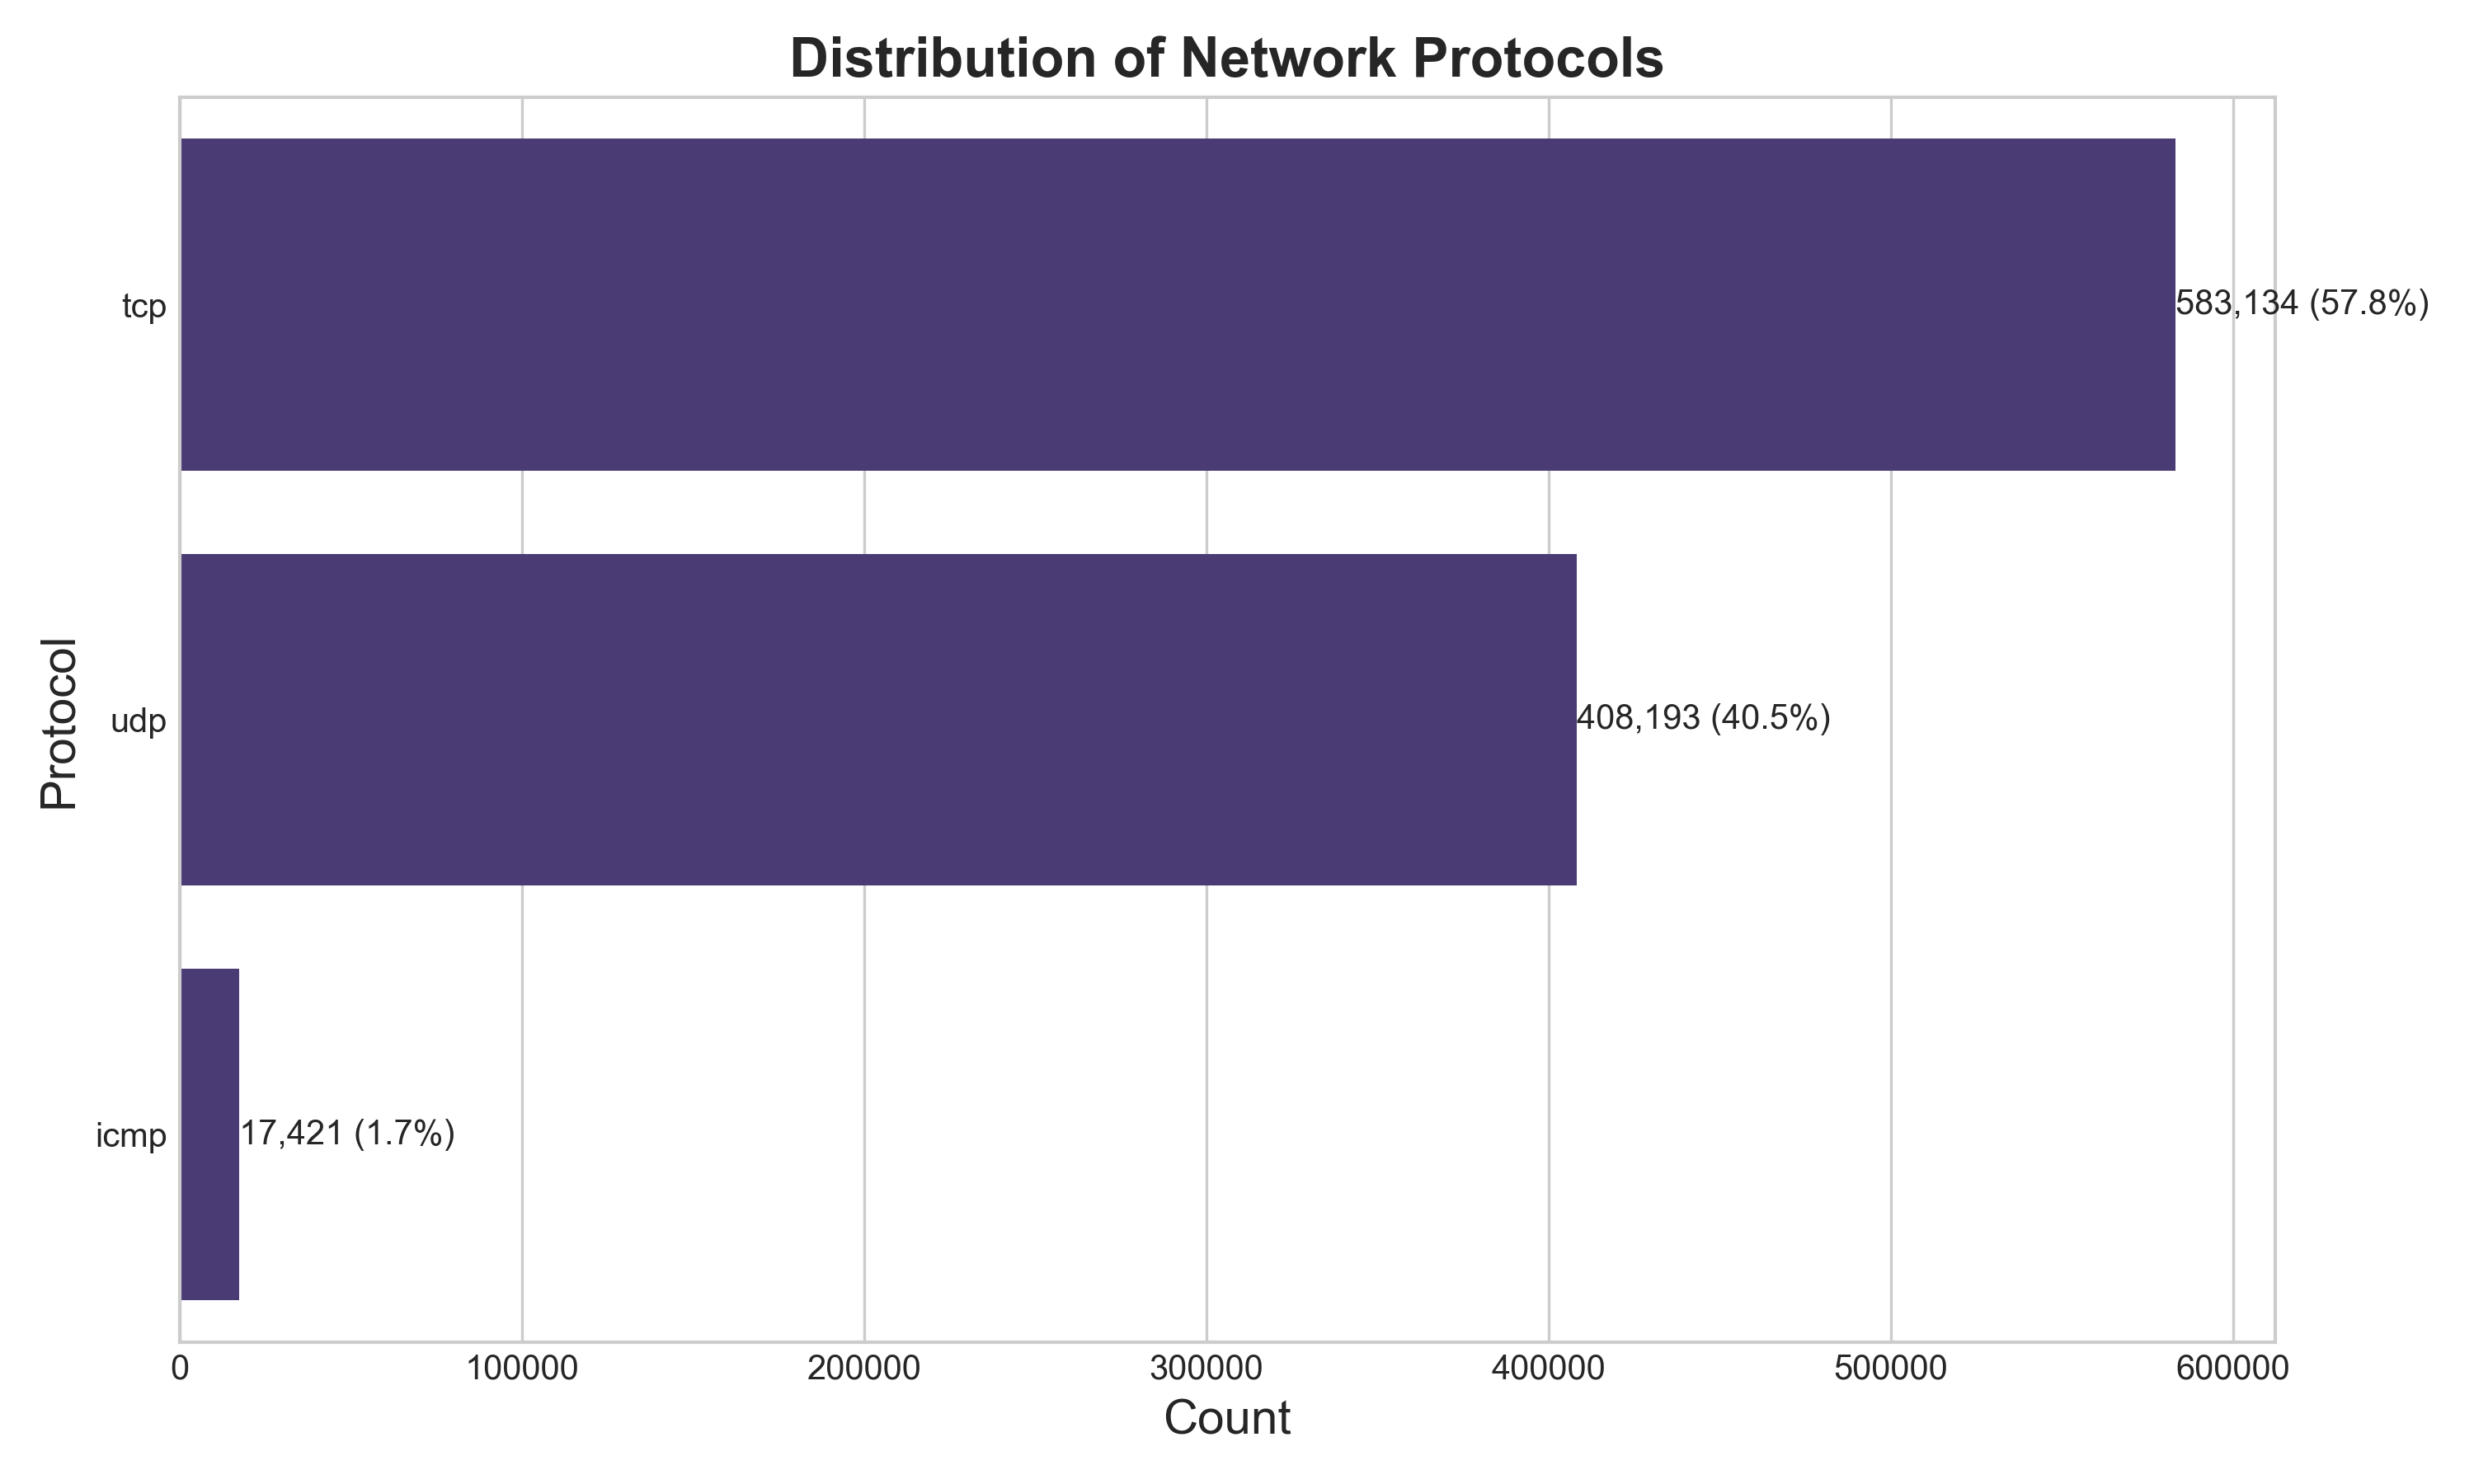
\includegraphics[width=\textwidth]{figures/protocol_distribution.png}
        \caption{Overall distribution of protocols.}
        \label{fig:protocol_distribution}
    \end{subfigure}
    \hfill % Adds horizontal space between the subfigures
    \begin{subfigure}[b]{0.48\textwidth}
        \centering
        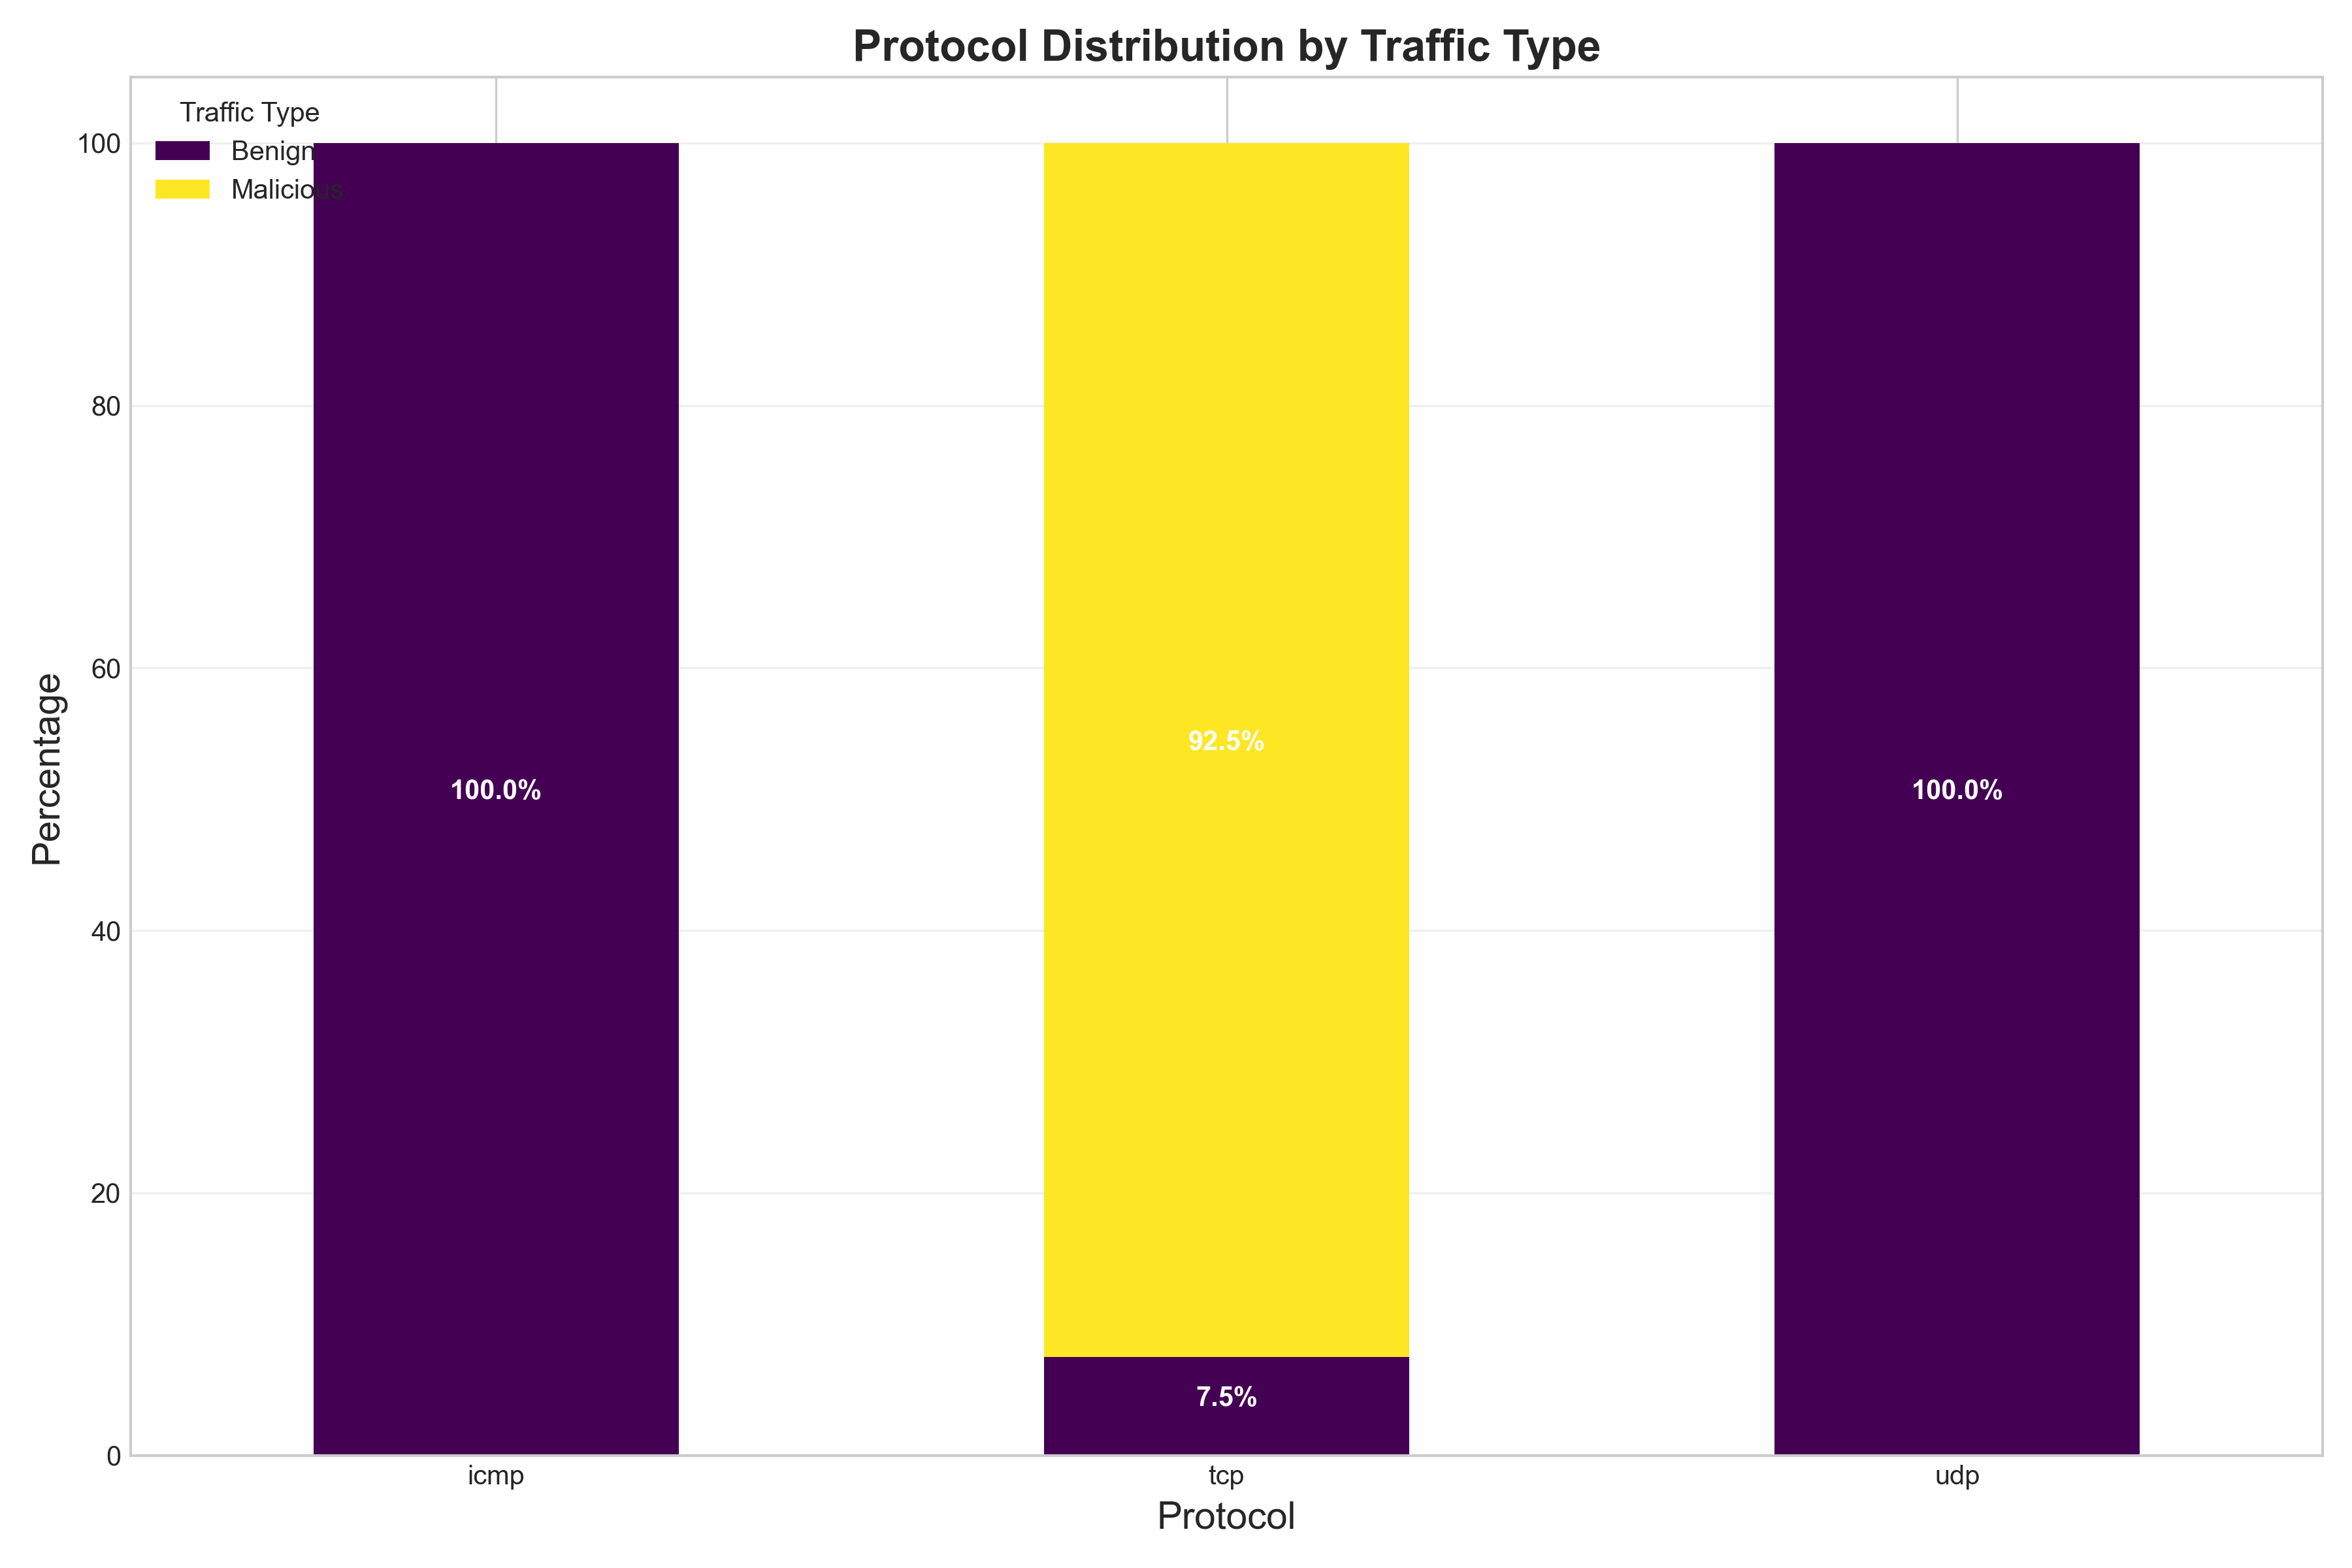
\includegraphics[width=\textwidth]{figures/protocol_by_label.png}
        \caption{Protocol distribution by traffic type.}
        \label{fig:protocol_by_label}
    \end{subfigure}
    
    \caption{Analysis of network protocols. TCP is the most common overall, but its prevalence differs significantly between malicious (72.4\%) and benign (40.9\%) traffic.}
    \label{fig:protocol_analysis} % A new label for the combined figure might be useful
\end{figure}

\paragraph{Connection State Analysis:}  
The connection state, particularly the S0 state (no response after a connection attempt), is a strong indicator of scanning activity. Figures~\ref{fig:connection_states} and \ref{fig:connection_states_by_label} demonstrate that while benign traffic features a balanced variety of connection states, 94.7\% of malicious connections exhibit the S0 state.

\begin{figure}[htbp]
    \centering
    \begin{subfigure}[b]{0.48\textwidth}
        \centering
        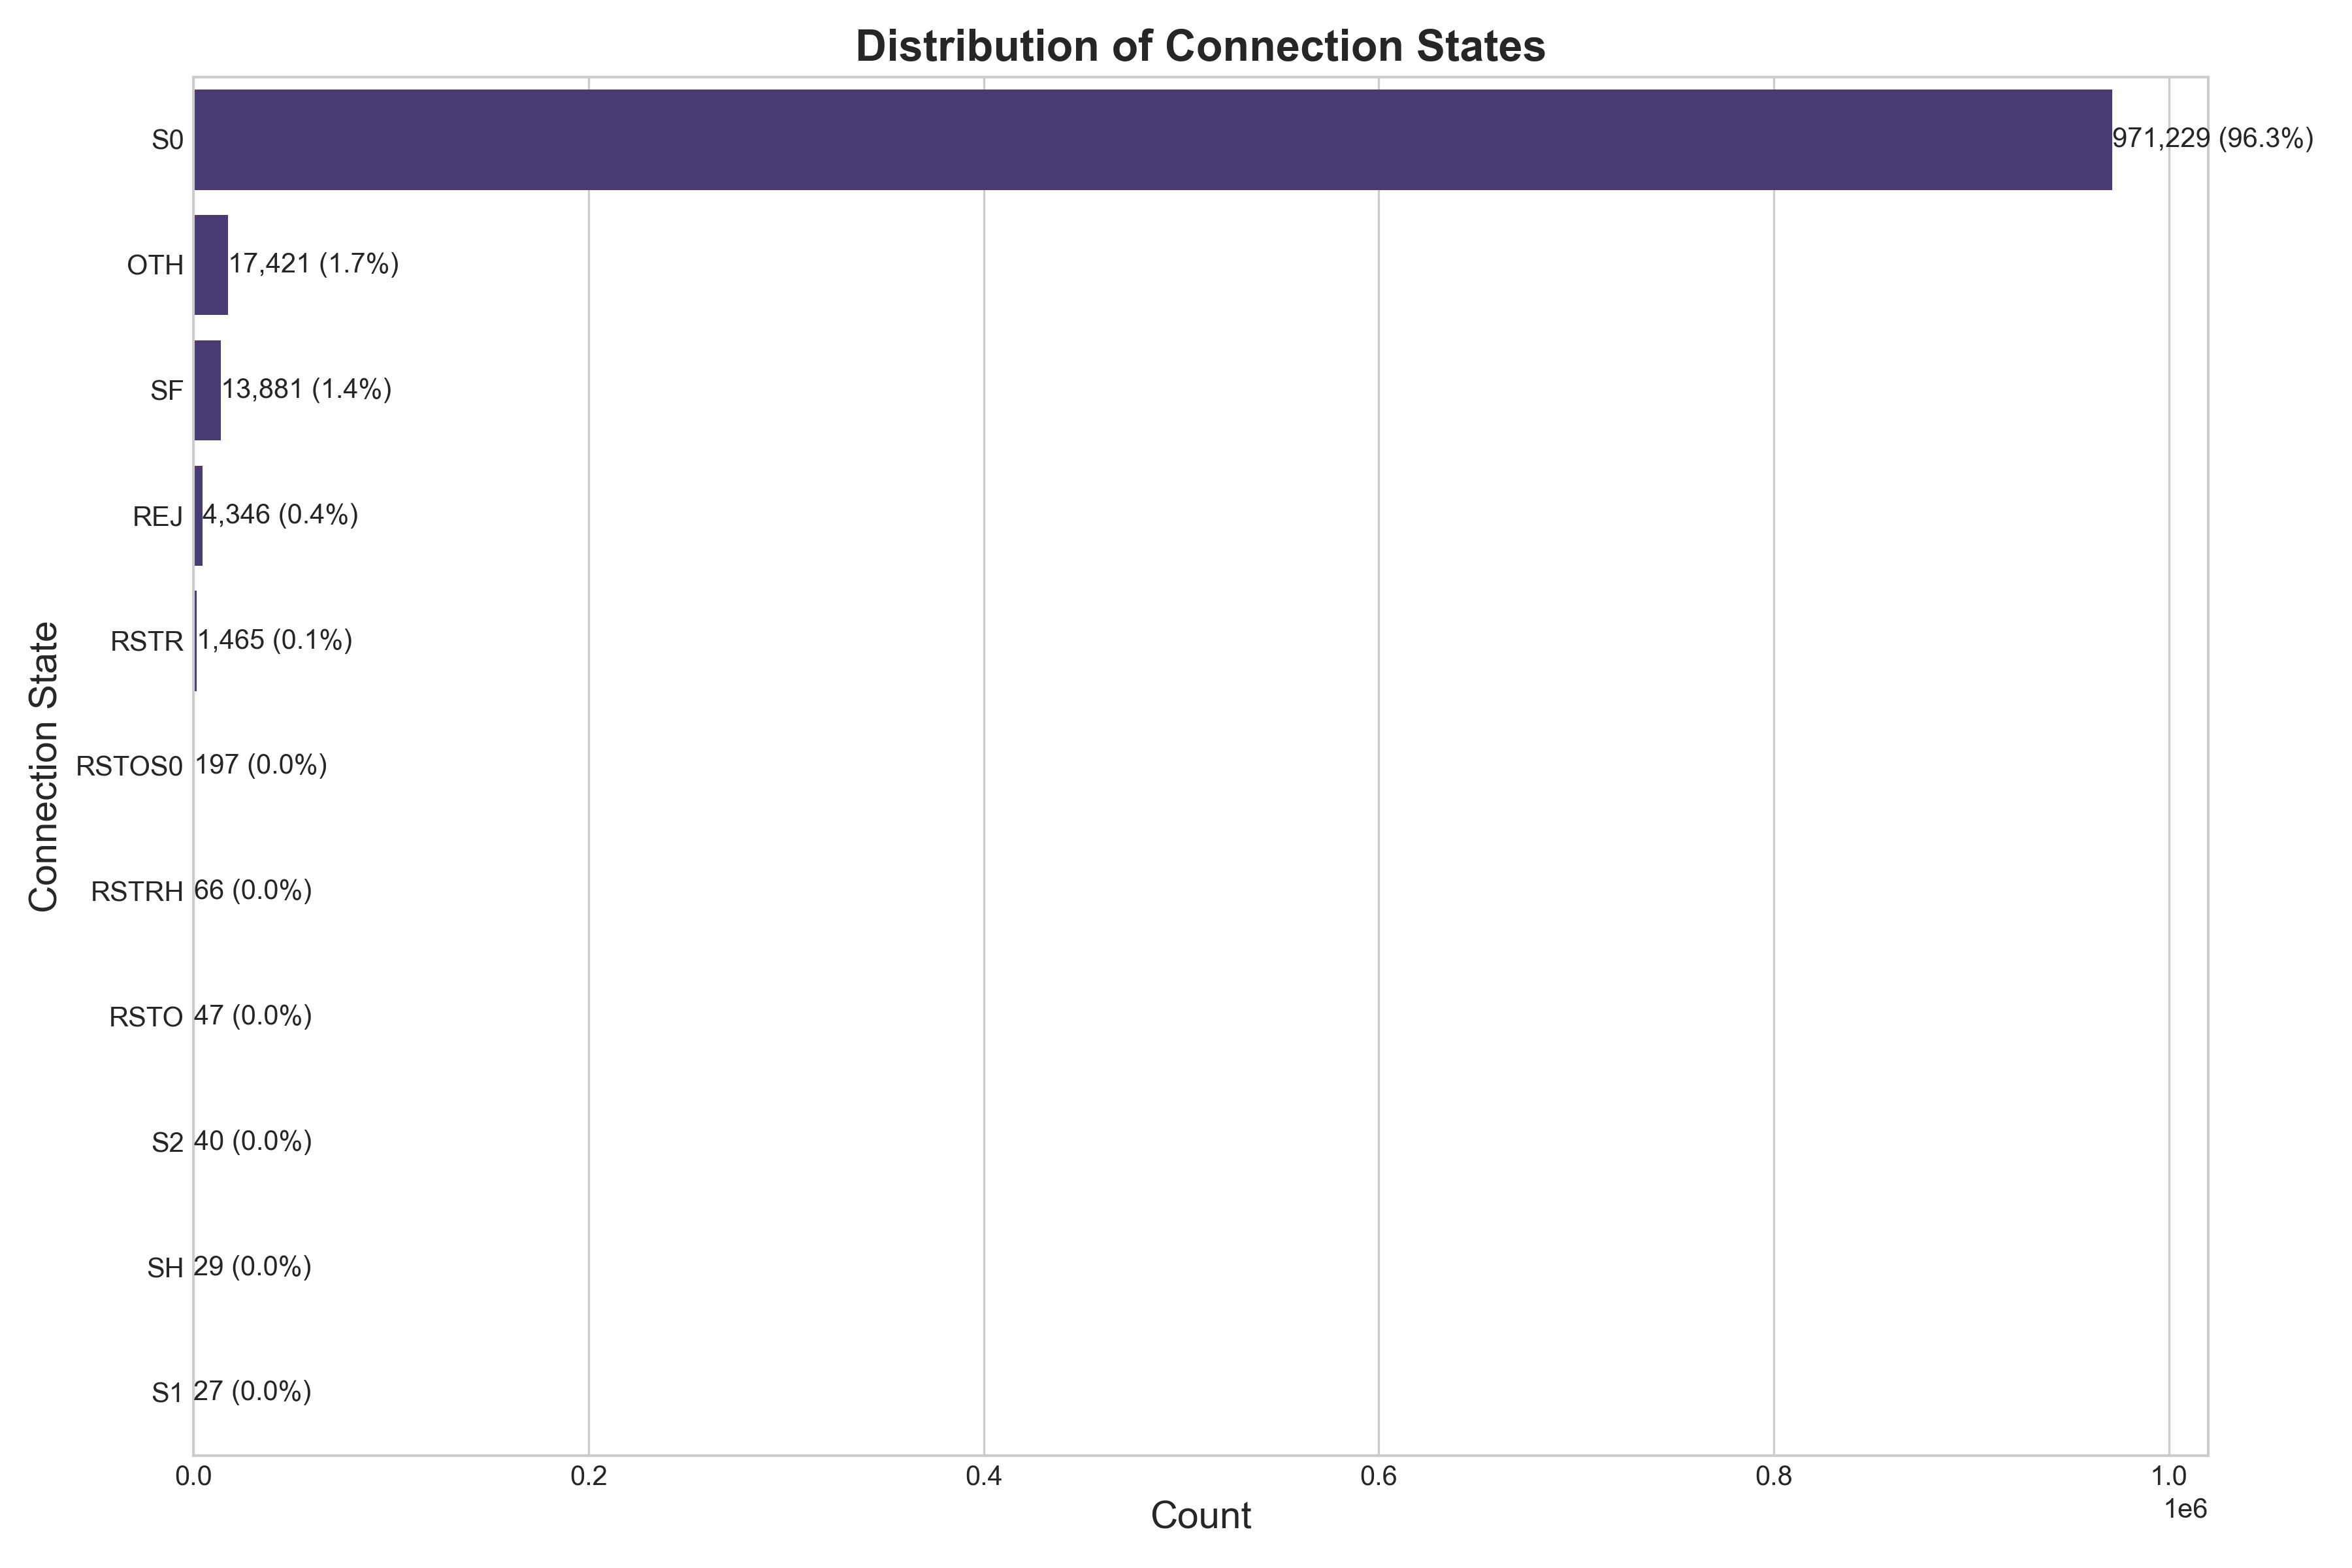
\includegraphics[width=\textwidth]{figures/connection_states.png}
        \caption{Overall distribution of connection states.}
        \label{fig:connection_states}
    \end{subfigure}
    \hfill % Adds horizontal space between the subfigures
    \begin{subfigure}[b]{0.48\textwidth}
        \centering
        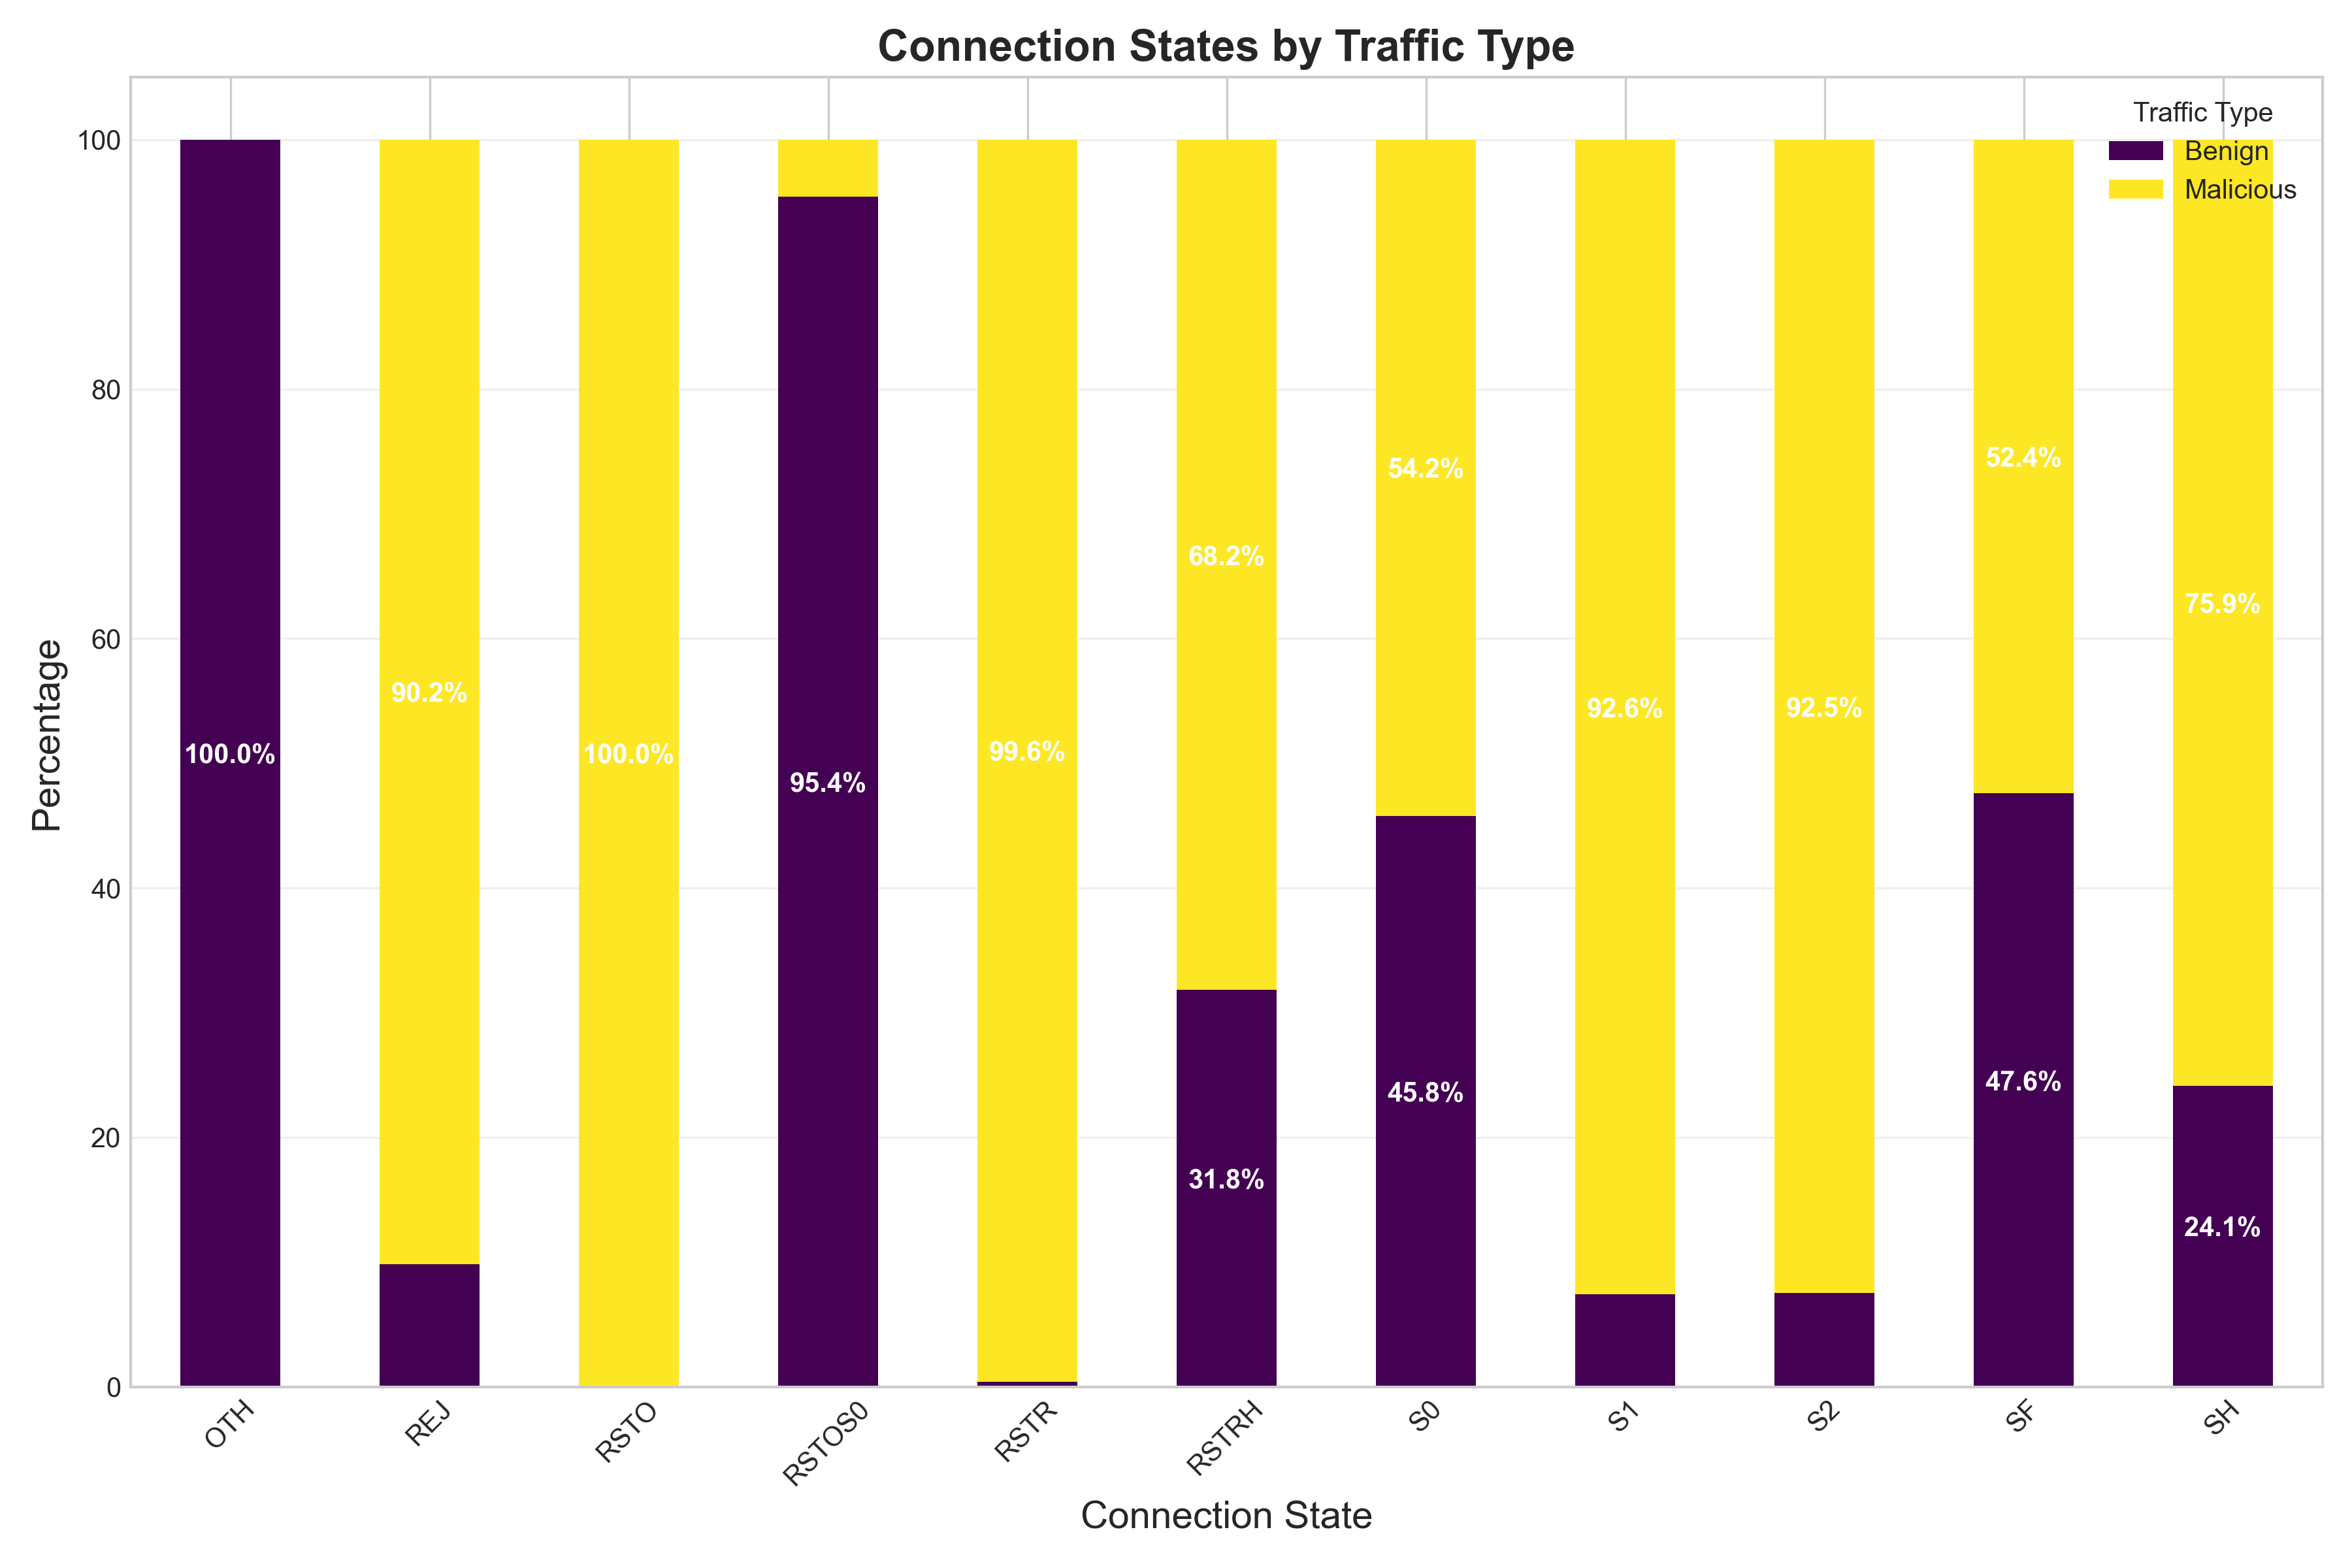
\includegraphics[width=\textwidth]{figures/connection_states_by_label.png}
        \caption{Connection states by traffic type.}
        \label{fig:connection_states_by_label}
    \end{subfigure}
    
    \caption{Analysis of connection states. The S0 state (connection attempt without response) dominates malicious traffic (94.7\%), indicating scanning activity, while benign traffic shows a diverse range of states.}
    \label{fig:connection_states_analysis} % A new label for the combined figure might be useful
\end{figure}


\paragraph{Temporal Analysis:}  
Temporal patterns, as seen in Figure~\ref{fig:hourly_traffic}, reveal that benign traffic follows a typical diurnal pattern with peak activity during working hours. In contrast, malicious traffic occurs in concentrated bursts, suggesting the use of automated scanning tools that operate in batches to evade detection.

\begin{figure}[htbp]
    \centering
    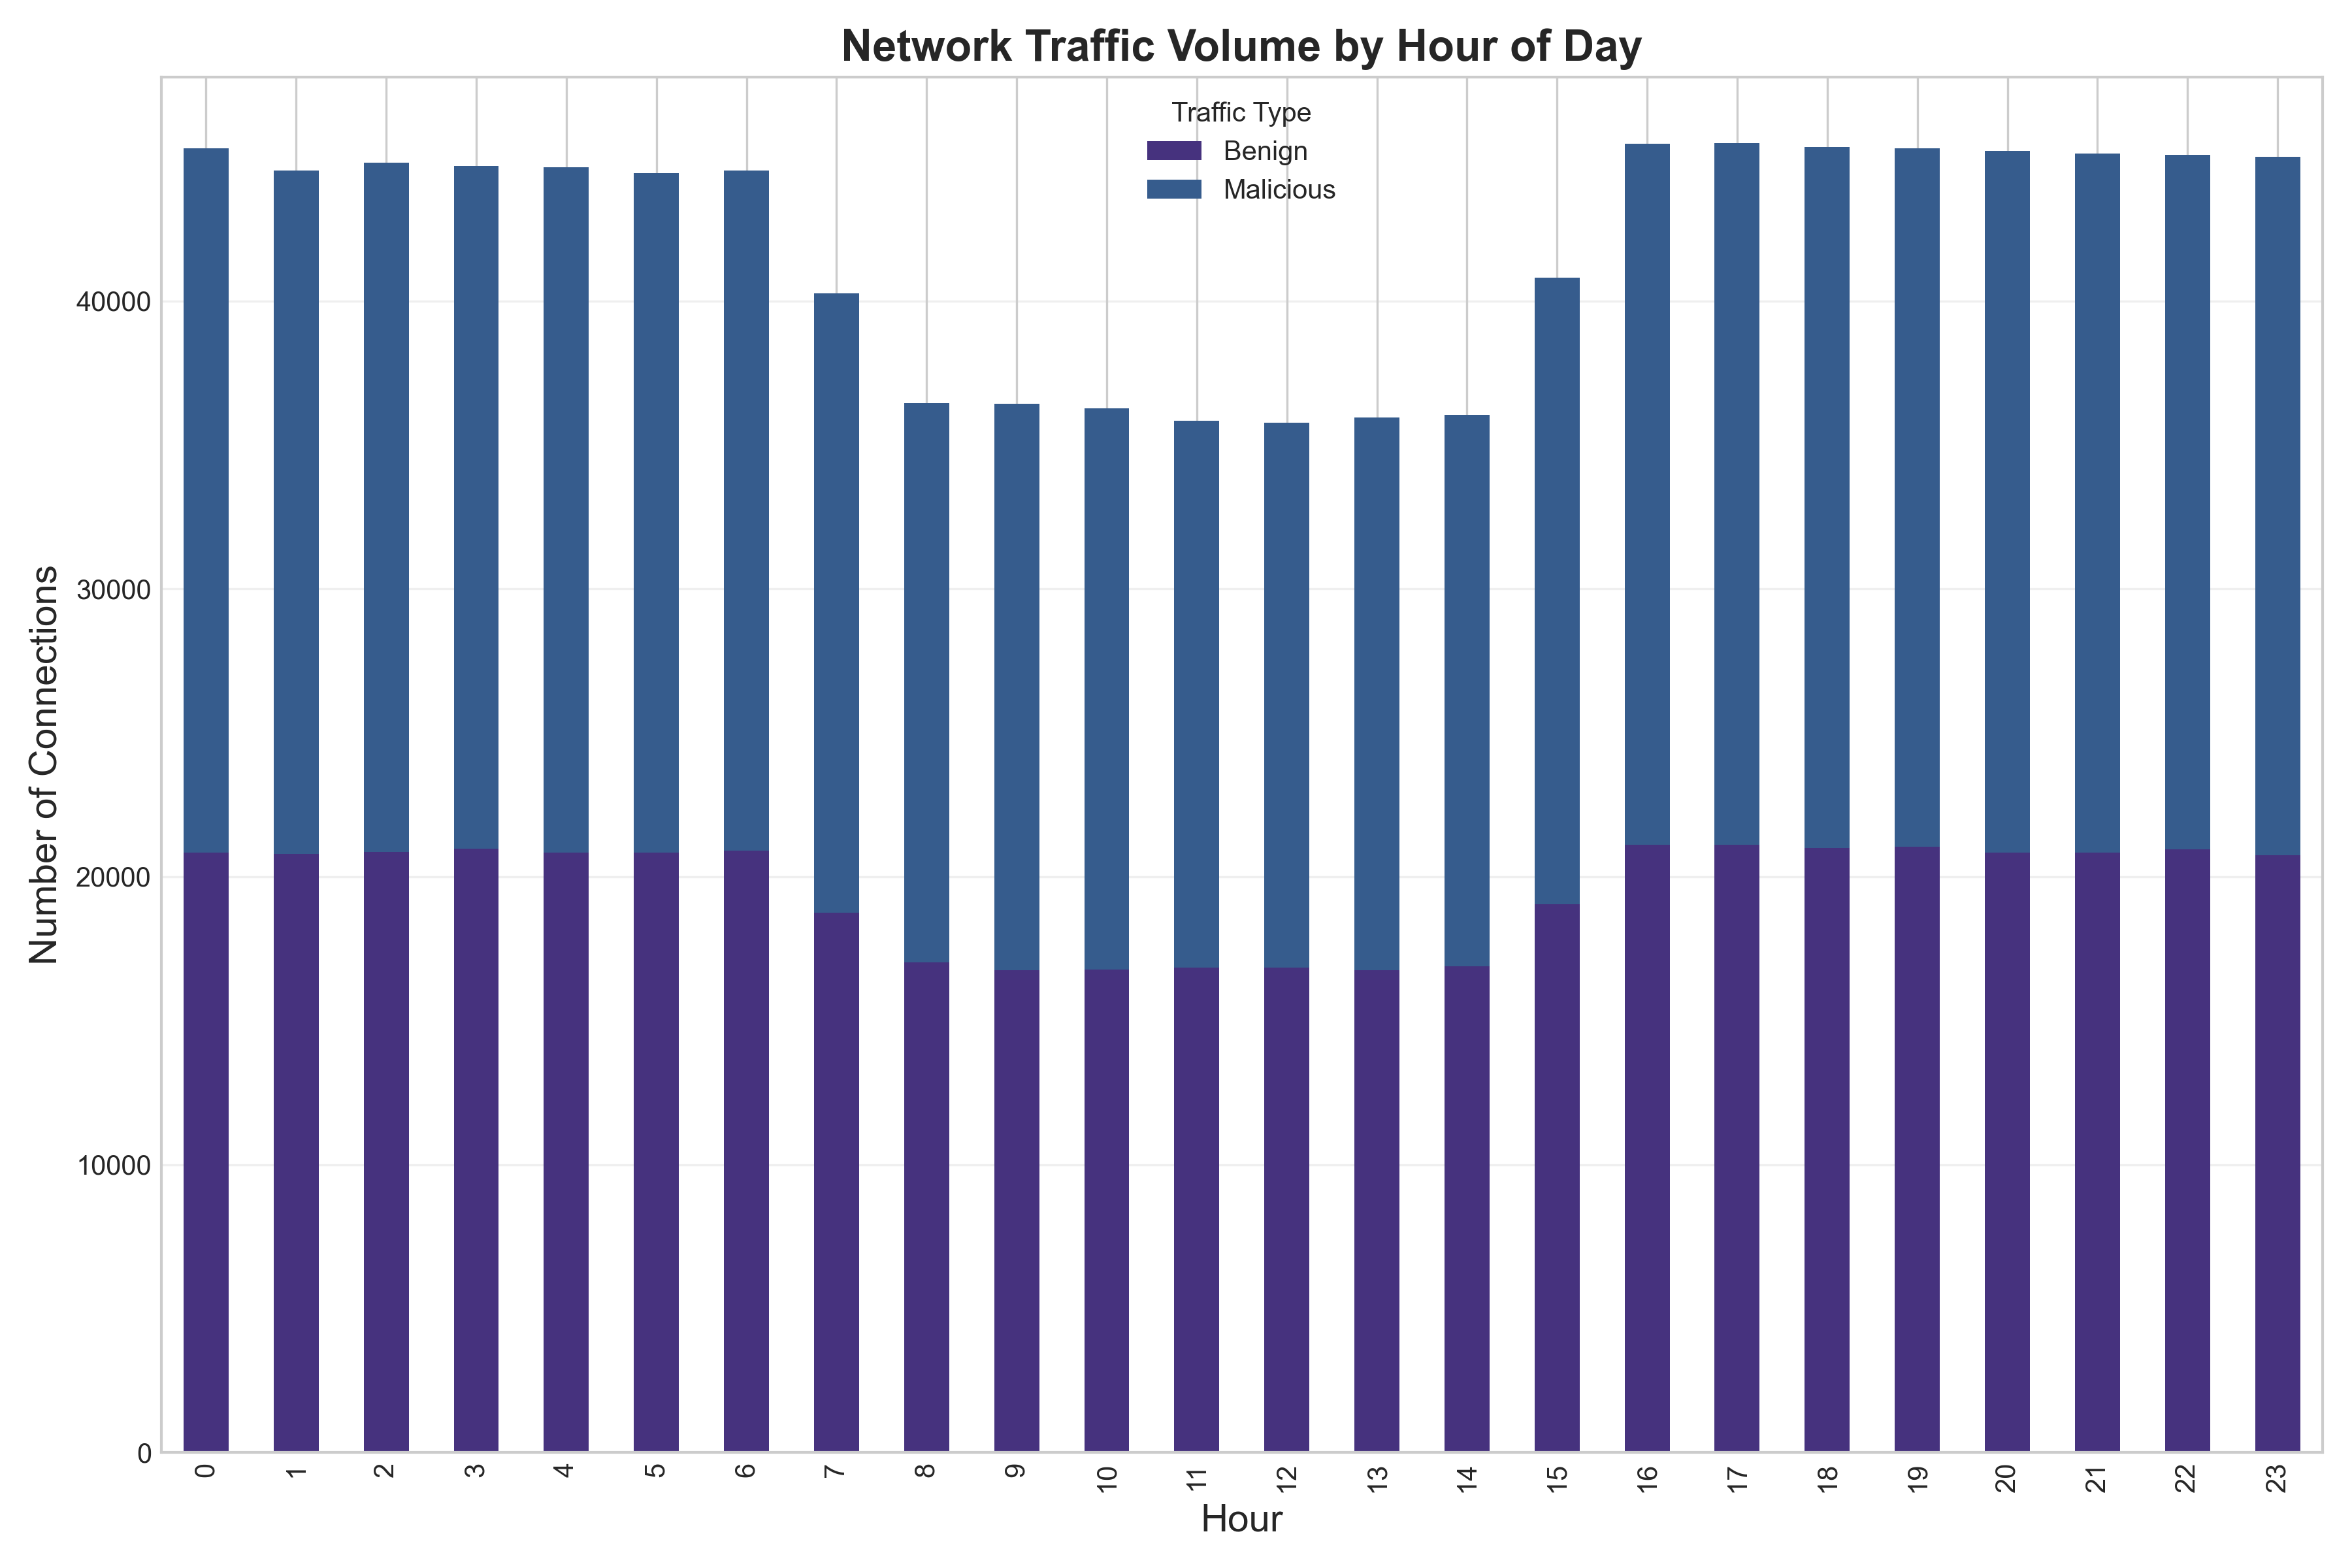
\includegraphics[width=\textwidth]{figures/hourly_traffic.png}
    \caption{Hourly distribution of network traffic, highlighting the diurnal pattern of benign traffic and the burst activity of malicious traffic.}
    \label{fig:hourly_traffic}
\end{figure}



\paragraph{Traffic Feature Analysis:}  
Additional analysis of data transfer volumes (Figure~\ref{fig:bytes_distribution}) and the relationship between packet counts and bytes transferred (Figure~\ref{fig:packets_vs_bytes}) shows that malicious traffic generally involves minimal data exchange. Such characteristics are consistent with scanning behaviour and form a key part of the feature set used for classification.

\begin{figure}[htbp]
    \centering
    \begin{subfigure}[b]{0.48\textwidth}
        \centering
        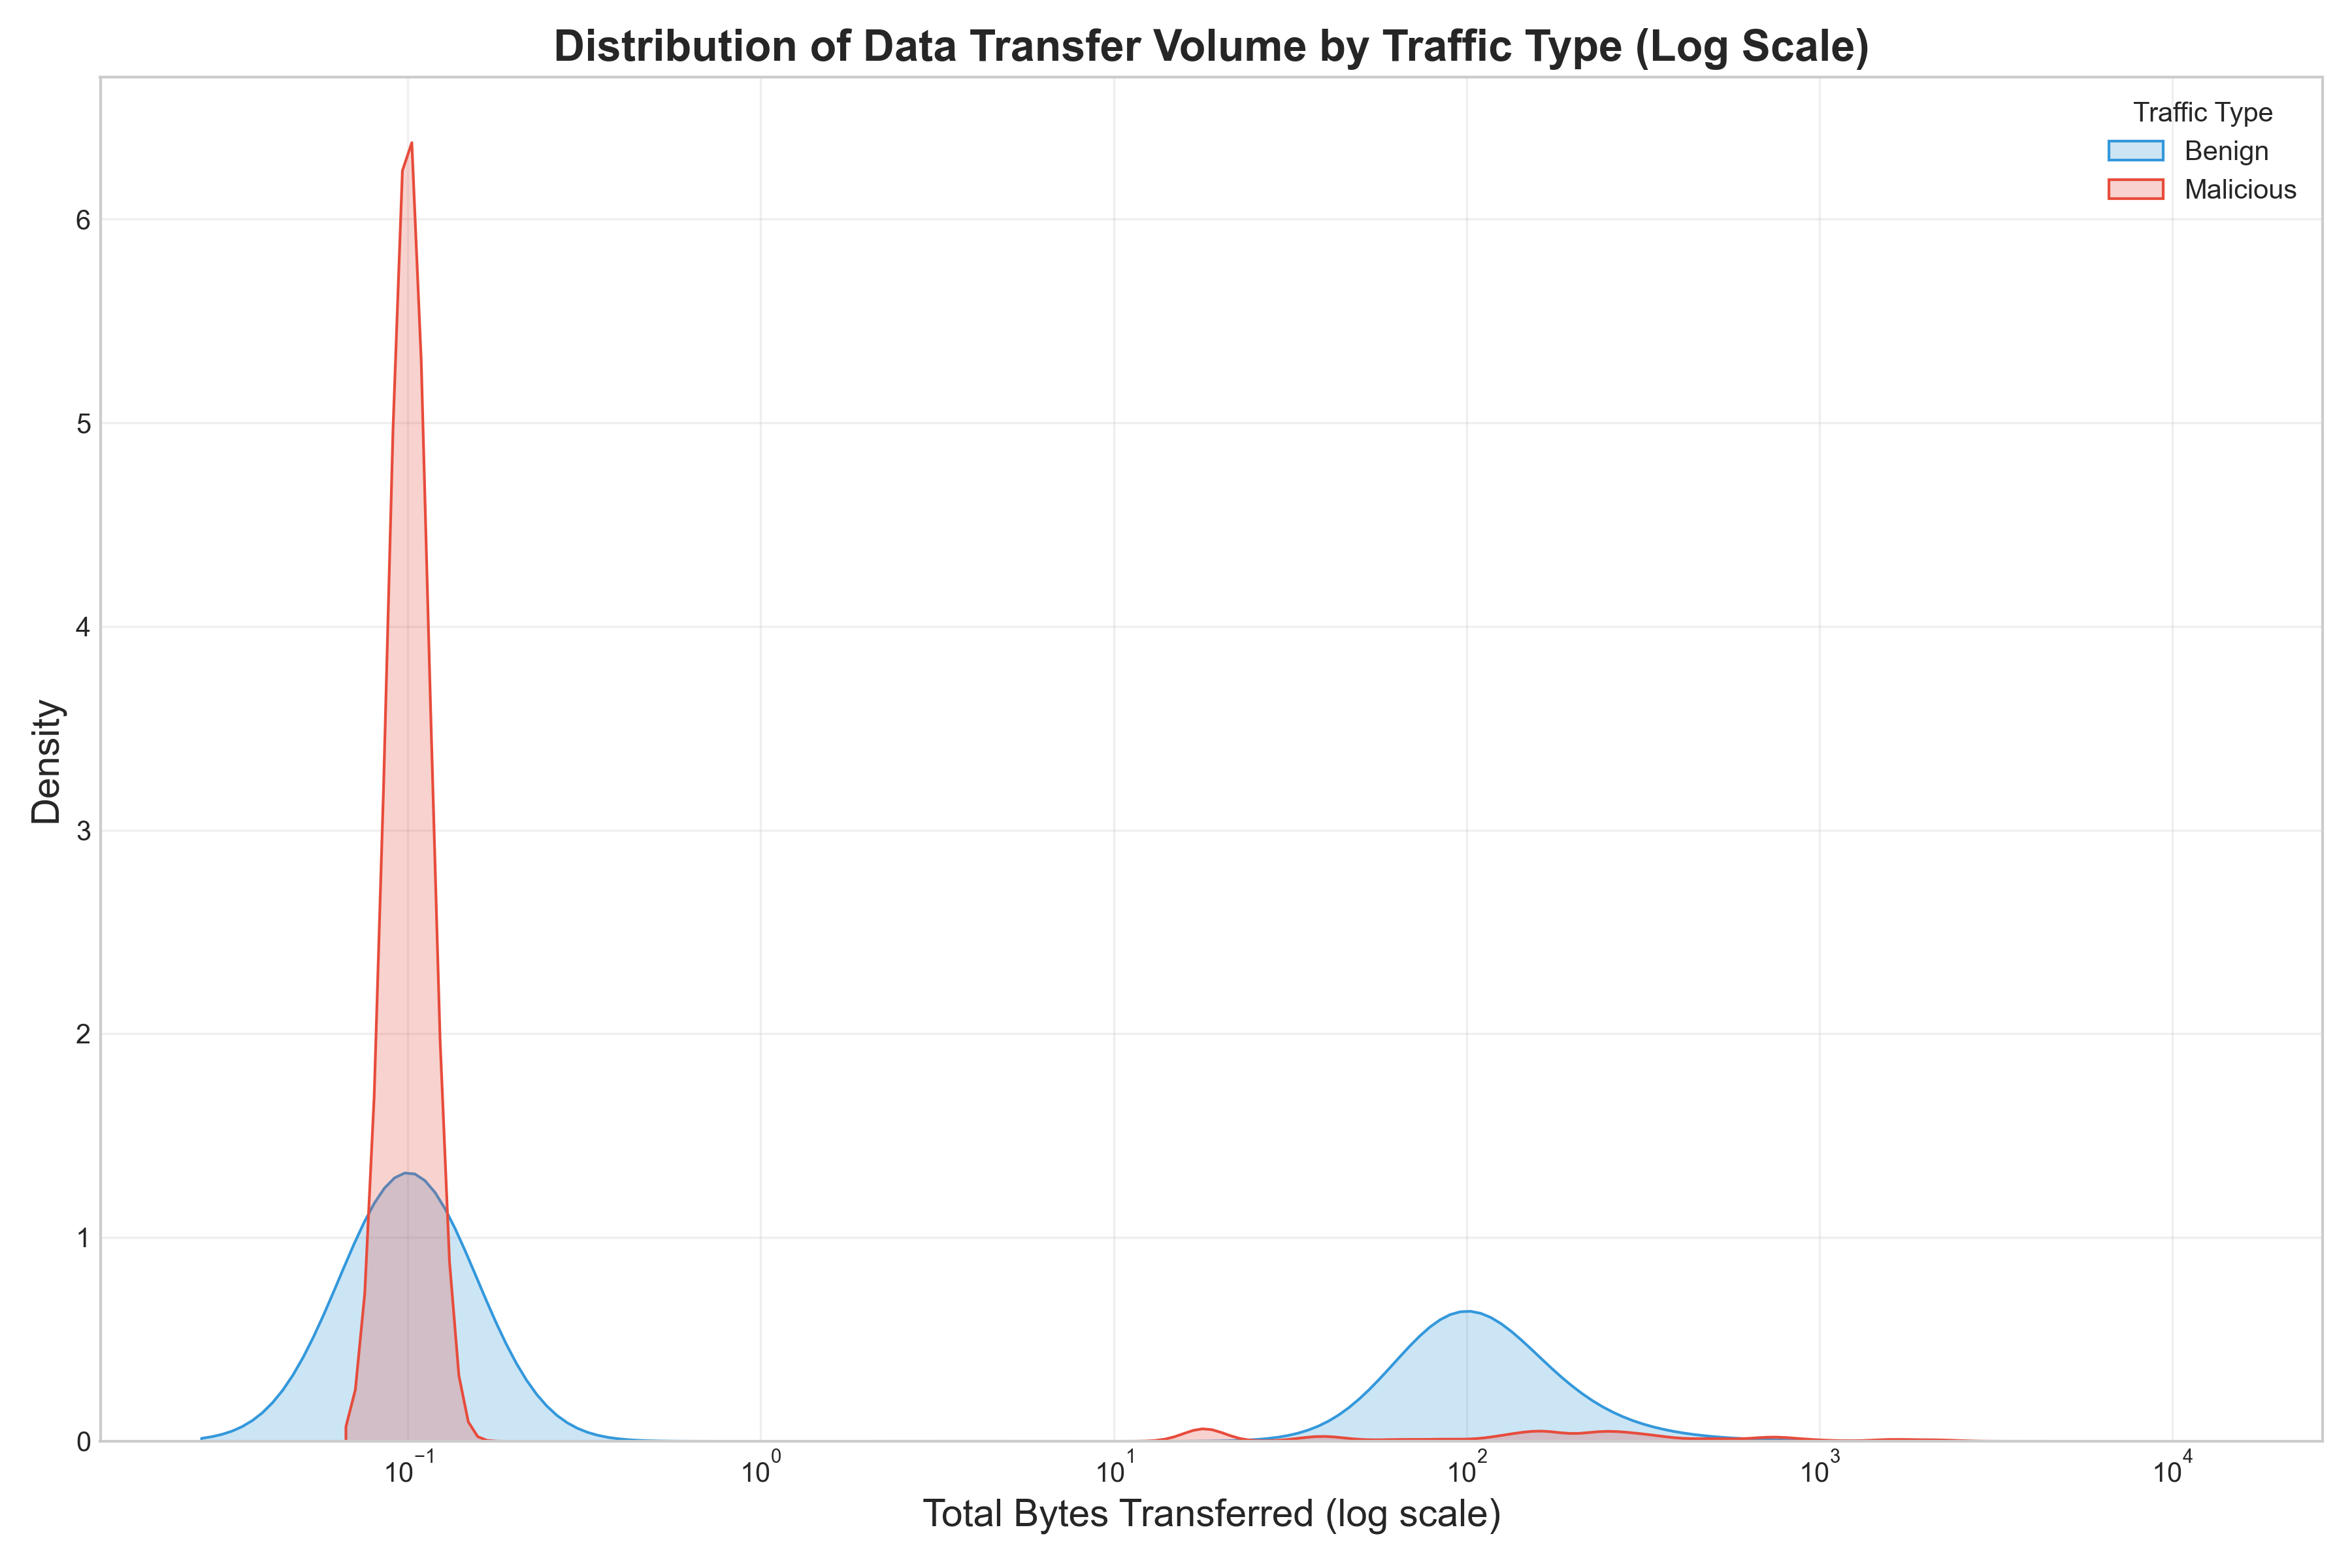
\includegraphics[width=\textwidth]{figures/bytes_distribution.png}
        \caption{Distribution of bytes transferred.}
        \label{fig:bytes_distribution}
    \end{subfigure}
    \hfill % Adds horizontal space between the subfigures
    \begin{subfigure}[b]{0.48\textwidth}
        \centering
        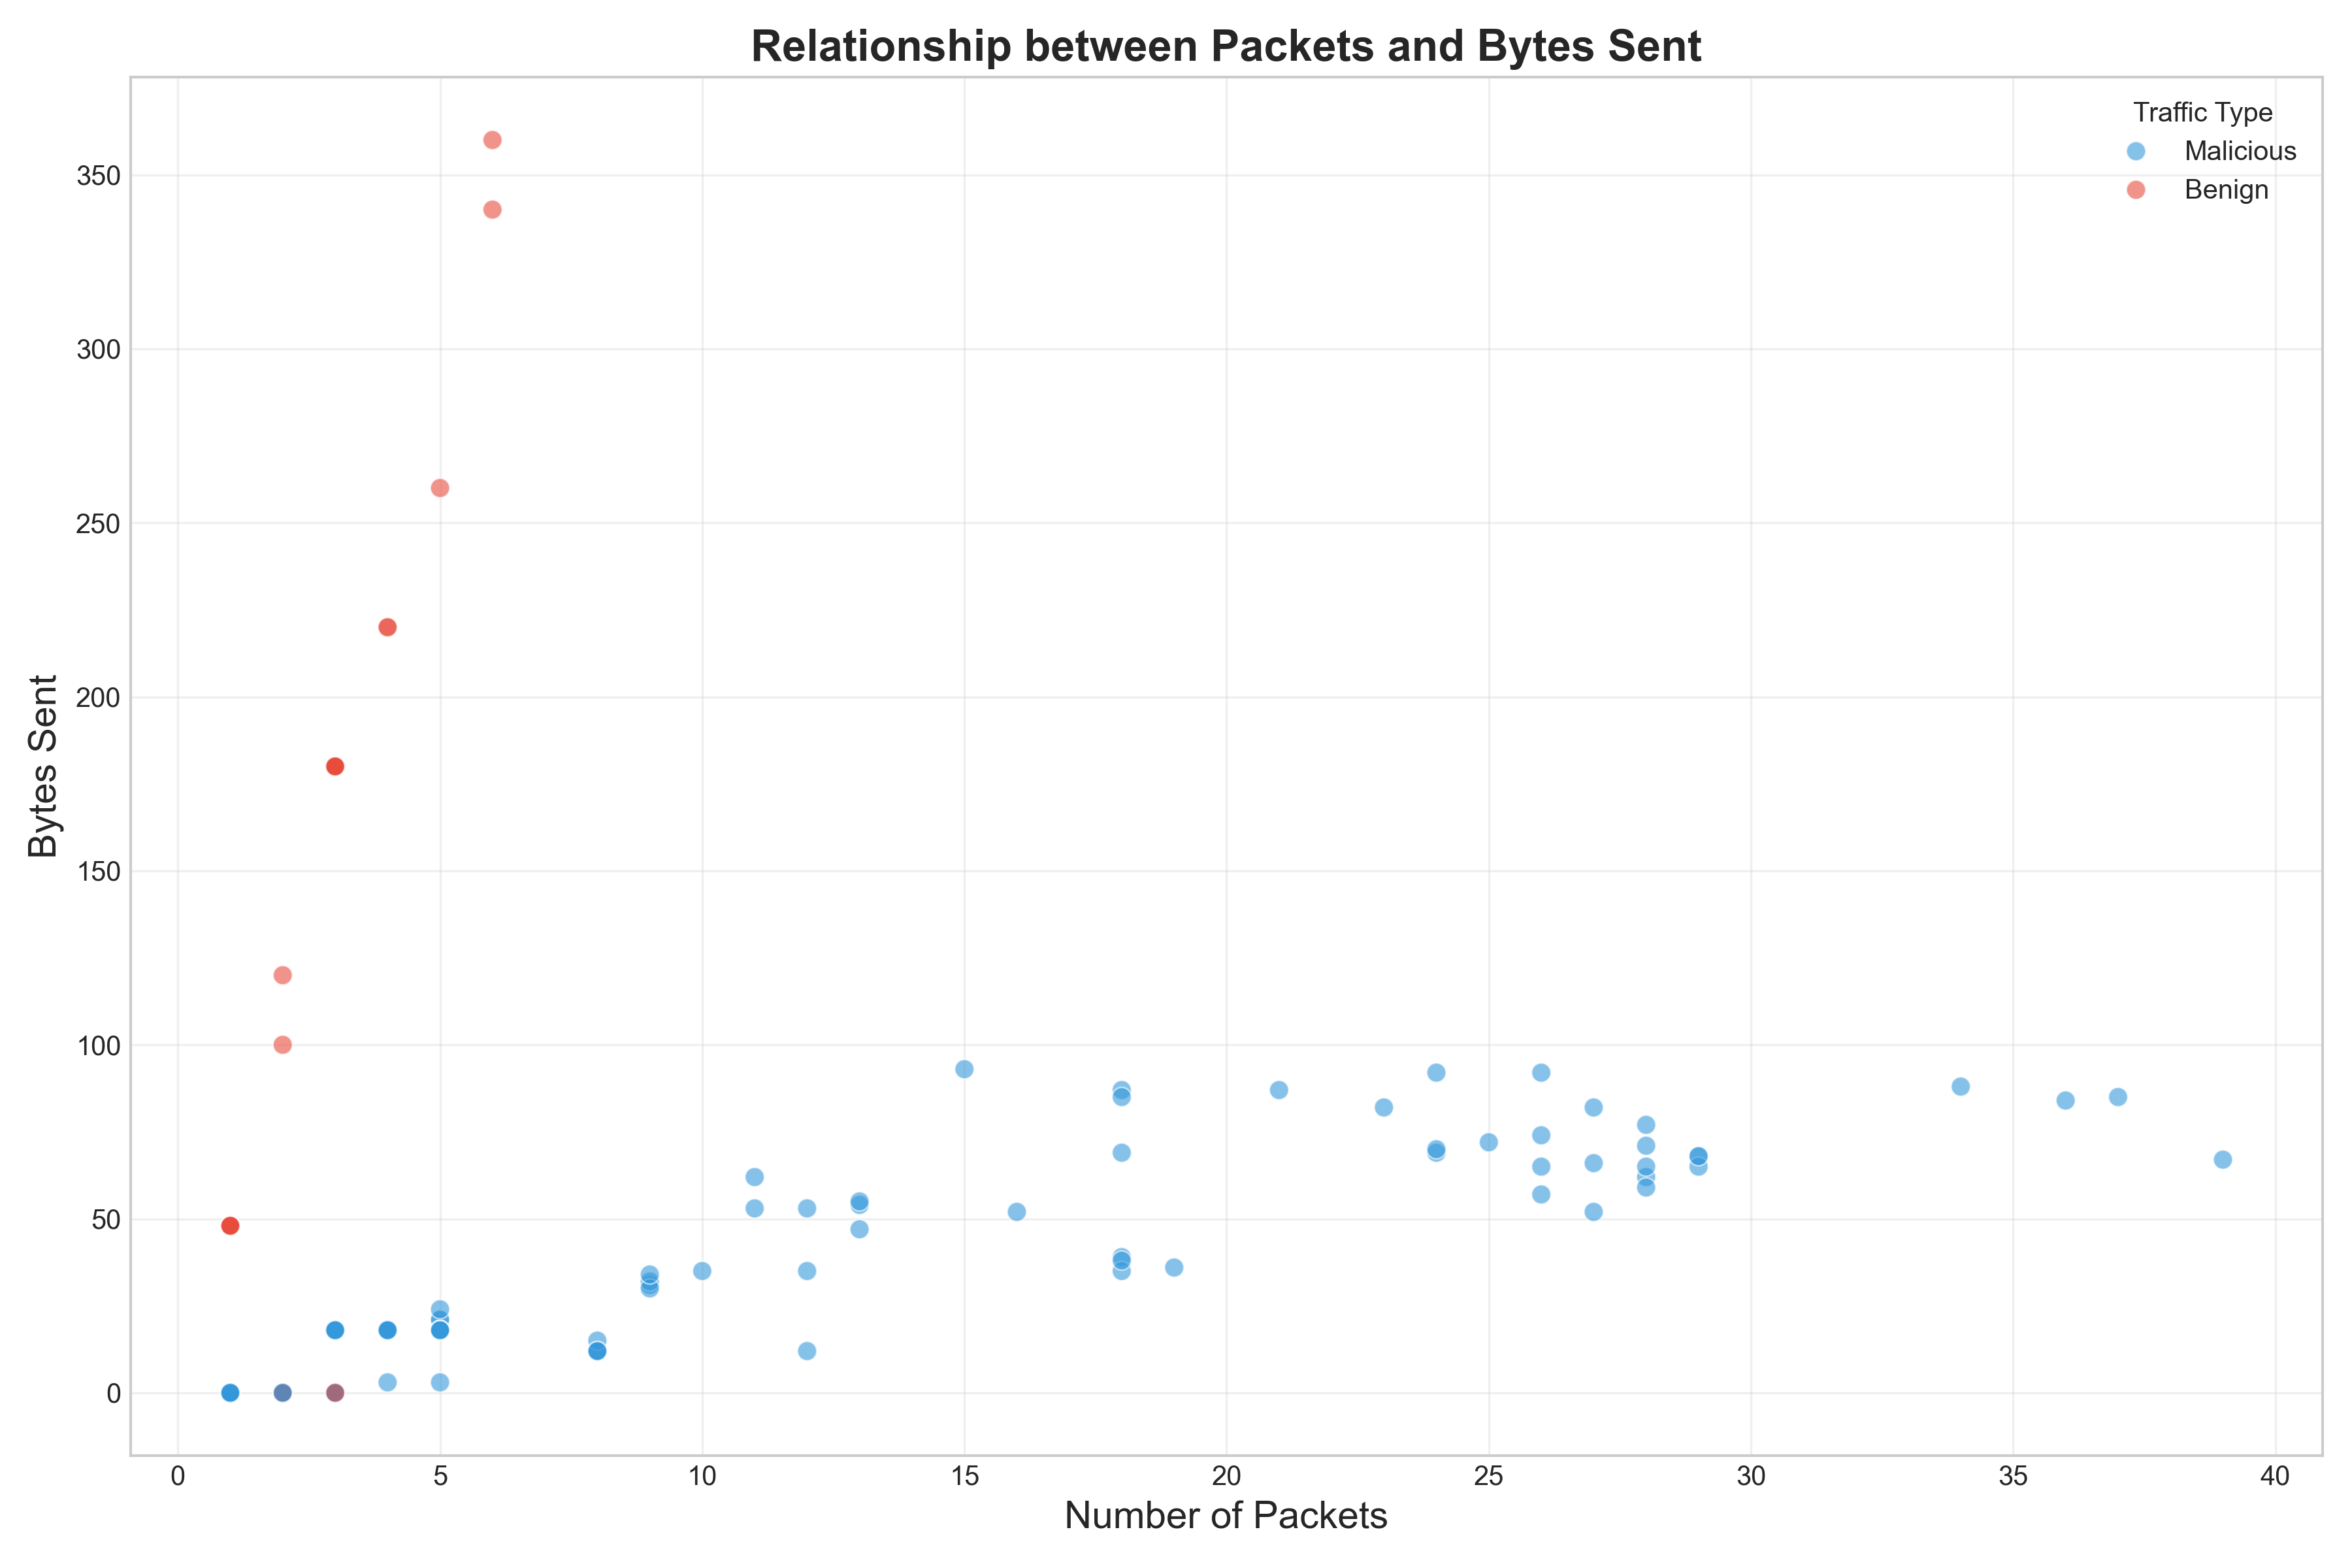
\includegraphics[width=\textwidth]{figures/packets_vs_bytes.png}
        \caption{Packets versus bytes transferred.}
        \label{fig:packets_vs_bytes}
    \end{subfigure}
    
    \caption{Analysis of traffic volume characteristics. Malicious traffic generally involves minimal data exchange, consistent with scanning behaviour.}
    \label{fig:traffic_volume_analysis} % A new label for the combined figure
\end{figure}


\paragraph{Feature Correlation:}
The correlation matrix (Figure~\ref{fig:correlation_matrix}) indicates that several features are highly correlated, particularly those related to connection states and traffic volume. This multicollinearity can affect model performance, necessitating careful feature selection and dimensionality reduction.

\begin{figure}[htbp]
    \centering
    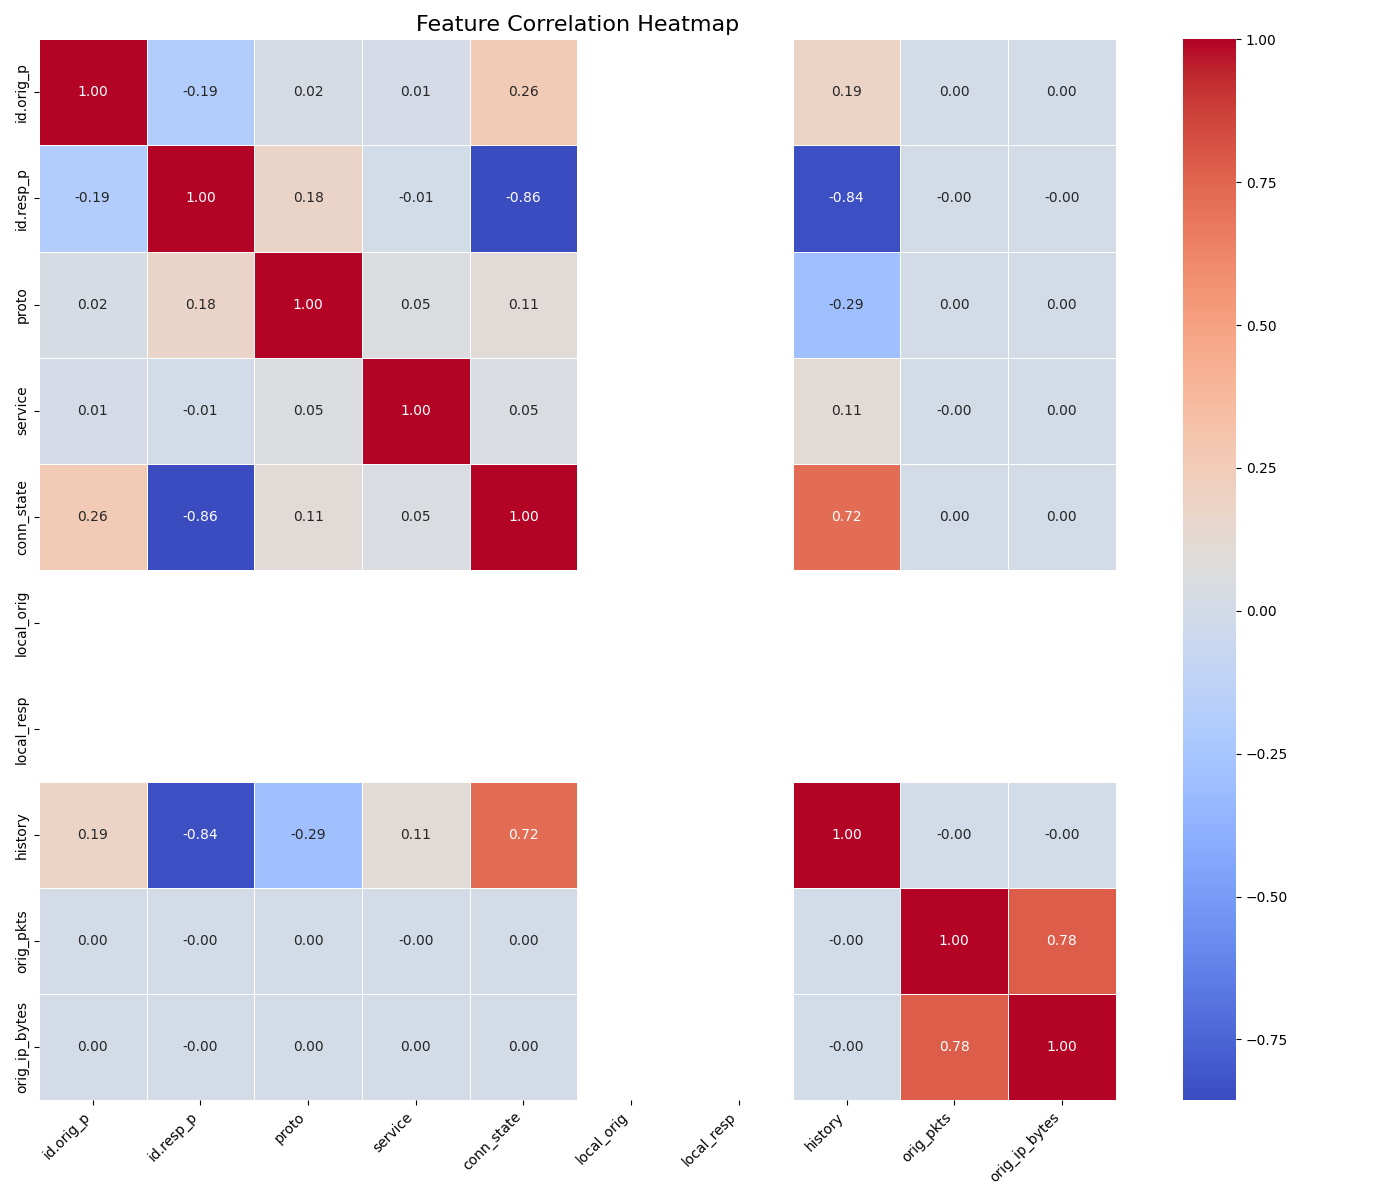
\includegraphics[width=\textwidth]{figures/feature_correlation.png}
    \caption{Correlation matrix of the top features, highlighting multicollinearity among connection states and traffic volume metrics.}
    \label{fig:correlation_matrix}
\end{figure}



\paragraph{Dimensionality Reduction:}  
Principal Component Analysis (PCA) was applied to the normalised feature set. The resulting visualisation (Figure~\ref{fig:pca_visualization}) confirms that the extracted features create distinct clusters for benign and malicious traffic. The first two principal components capture approximately 67\% of the variance, with features such as connection state, protocol type, and packet-to-byte ratios contributing most significantly.

\begin{figure}[htbp]
    \centering
    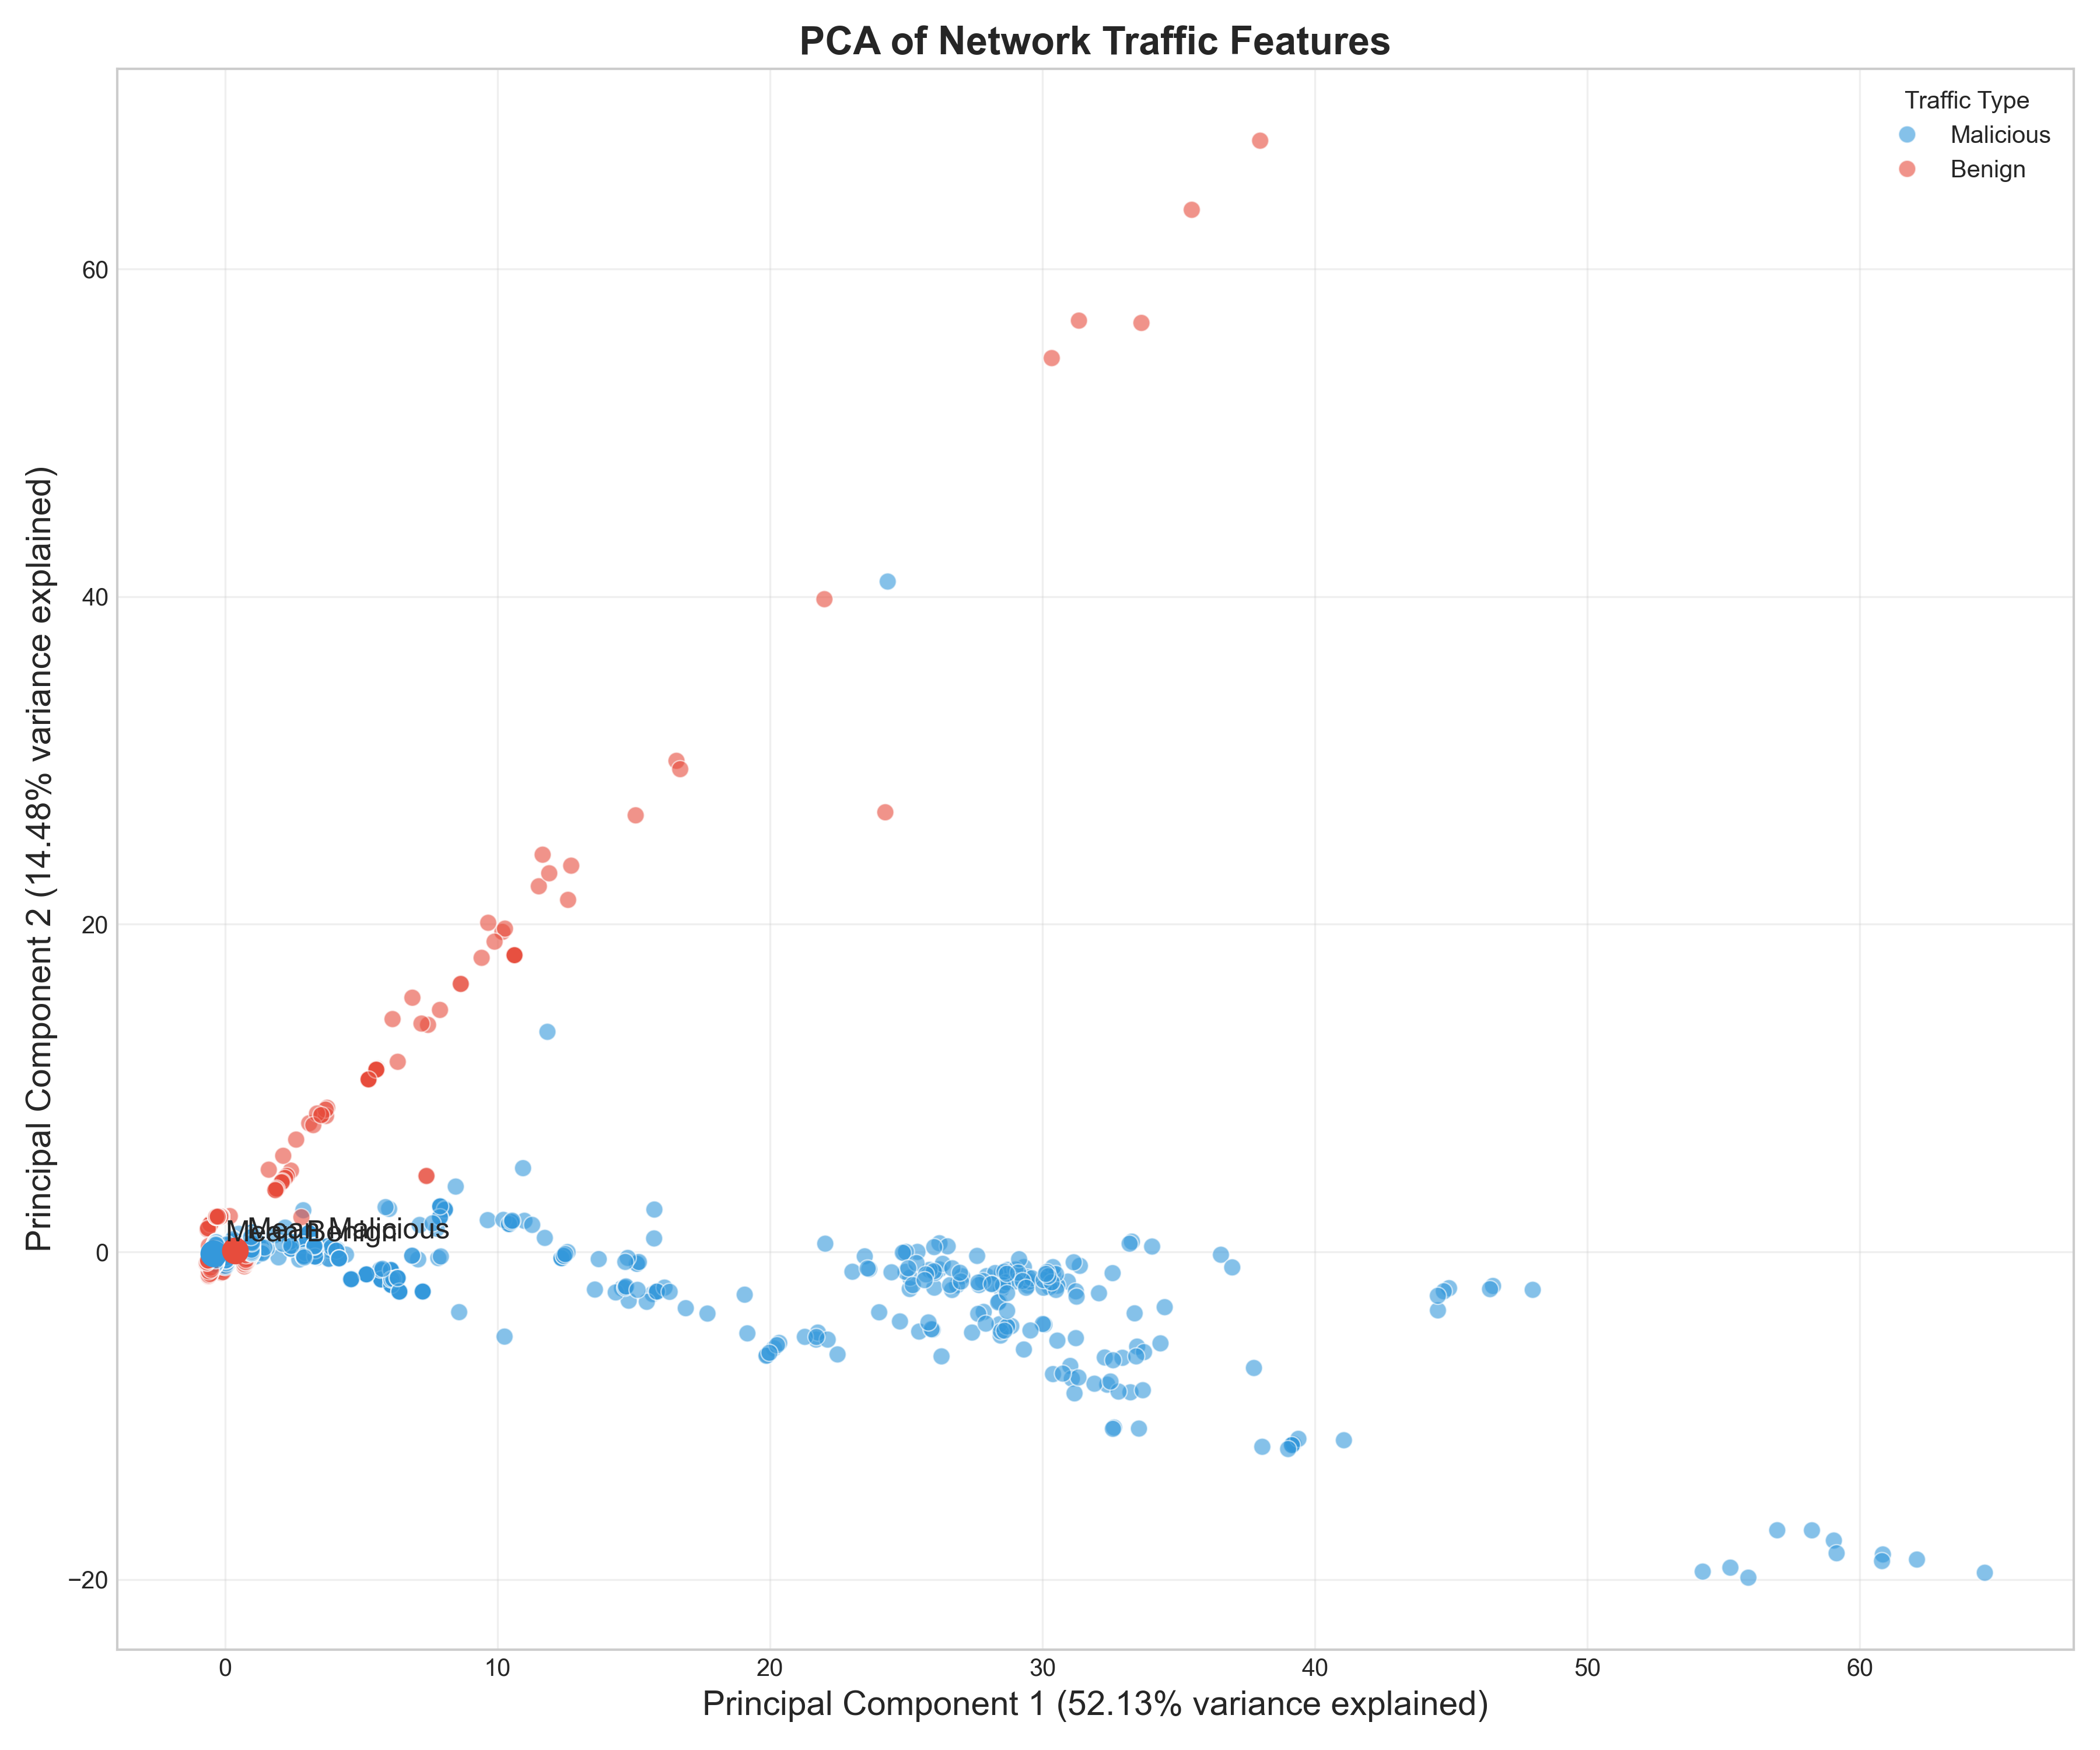
\includegraphics[width=\textwidth]{figures/pca_visualization.png}
    \caption{PCA visualisation of the feature space.}
    \label{fig:pca_visualization}
\end{figure} % Added missing \end{figure} to close the figure environment




\section{Machine Learning and Deep Learning Model Performance}

\subsection{Traditional Machine Learning Models}

A range of traditional machine learning models was evaluated for the malware detection task. Table~\ref{tab:model_performance} presents the performance metrics of the baseline Random Forest, XGBoost, and SVM models alongside their optimised versions.

\begin{table}[htbp]
    \center
    \begin{tabular}{lcccc}
    \hline
    \textbf{Model} & \textbf{Accuracy} & \textbf{Precision} & \textbf{Recall} & \textbf{F1-Score} \\
    \hline
    Random Forest             & 99.21\% & 99.15\% & 99.23\% & 99.19\% \\
    XGBoost                   & 99.17\% & 99.12\% & 99.18\% & 99.15\% \\
    SVM                       & 98.73\% & 98.45\% & 98.91\% & 98.68\% \\
    Optimised Random Forest   & \textbf{99.96\%} & \textbf{99.92\%} & \textbf{100.00\%} & \textbf{99.96\%} \\
    Optimised XGBoost         & 99.89\% & 99.85\% & 99.90\% & 99.87\% \\
    \hline
    \end{tabular}
    \caption{Performance metrics for different machine learning models on the malware detection task.}
    \label{tab:model_performance}
\end{table}

Among the base models, Random Forest generally outperformed both XGBoost and SVM. This can be ascribed to its ensemble nature and its ability to handle mixed data types without extensive preprocessing. The application of hyperparameter optimisation, for instance through RandomisedSearchCV, further enhanced model performance. The optimised Random Forest achieved near-perfect classification with 99.96\% accuracy and complete recall, ensuring that no malicious connection was overlooked.

Our evaluation of multiple machine learning approaches revealed several insights regarding algorithmic performance for malware detection in IoT network traffic. The exceptional performance achieved by all models (exceeding 98.5\% accuracy) demonstrates that machine learning is highly effective for this particular security application when it is provided with appropriate features.

\subsection{Feature Importance Insights}

Analysis of the importance of features of the optimised Random Forest model provided valuable insight into the detection process. Connection state features consistently ranked as the most influential predictors, followed by protocol information and traffic volume metrics.

Interestingly, while the temporal features individually showed moderate importance, their collective contribution was substantial. This suggests that malicious activity patterns manifest on multiple time-related dimensions that the model successfully integrated into its decision process.

The high importance of derived features (such as bytes-per-packet ratios and logarithmic transformations of traffic volumes) validates our feature engineering approach. These transformations helped capture the distinctive characteristics of scanning activities, which typically involve minimal data transfer and specific packet-size patterns.

\subsection{Hyperparameter Optimisation and Feature Importance}

The optimised models benefitted from several key adjustments:
\begin{itemize}
    \item \textbf{Tree structure adjustments:} Optimising tree depths and the minimum sample split parameters refined decision boundaries.
    \item \textbf{Ensemble size:} Increasing the number of trees improved stability and reduced variance.
    \item \textbf{Feature sampling:} Modifying feature sampling strategies enhanced the detection of subtle signals in less prominent features.
\end{itemize}

Table~\ref{tab:optimized_hyperparameters} illustrates the optimised hyperparameter configurations for the Random Forest and XGBoost models.

\begin{table}[htbp]
\centering
\caption{Optimised Hyperparameters for Random Forest and XGBoost Models}
\label{tab:optimized_hyperparameters}
\begin{tabular}{lcc}
\hline
\textbf{Hyperparameter} & \textbf{Random Forest} & \textbf{XGBoost} \\
\hline
max\_depth                & None (unlimited)       & 3              \\
min\_samples\_leaf        & 1                      & ---            \\
min\_samples\_split       & 10                     & ---            \\
n\_estimators            & 200                    & 100            \\
learning\_rate           & ---                    & 0.2            \\
colsample\_bytree        & ---                    & 0.8            \\
subsample                & ---                    & 1.0            \\
\hline
\end{tabular}
\end{table}

Feature importance analysis from the optimised Random Forest model confirmed that connection states, protocol information, and traffic volume metrics are pivotal for classification. This insight reinforces the efficacy of the feature engineering strategy, especially when combined with dimensionality reduction techniques such as PCA.

\subsection{Deep Learning Approach}

In addition to traditional models, a deep neural network was implemented to capitalise on the same set of network features. The architecture comprised:
\begin{itemize}
    \item An input layer with 18 features.
    \item Three hidden layers with 128, 64, and 32 neurons, each employing ReLU activation, batch normalisation, and a dropout rate of 30\%.
    \item An output layer with a sigmoid activation function for binary classification.
\end{itemize}

Trained with binary cross-entropy loss and the Adam optimiser (learning rate 0.001), the neural network achieved an accuracy of 99.77\%, as detailed in Table~\ref{tab:nn_performance}.

\begin{table}[ht]
\center
\begin{tabular}{lcccc}
\hline
\textbf{Model} & \textbf{Accuracy} & \textbf{Precision} & \textbf{Recall} & \textbf{F1-Score} \\
\hline
Neural Network    & 99.77\% & 99.75\% & 99.90\% & 99.82\% \\
\hline
\end{tabular}
\caption{Performance metrics for the neural network model on the malware detection task.}
\label{tab:nn_performance}
\end{table}

Comparison with traditional methods indicates that while the optimised Random Forest slightly outperforms the neural network in terms of accuracy, the deep learning model demonstrates notable benefits in interpretability through its direct probability outputs and robustness across evaluation metrics.

\section{Discussion of Findings and Implications for Malware Detection}

The integrated analysis confirms that network flow characteristics alone can yield exceptionally reliable malware detection. The following discussion summarises key insights:

\begin{itemize}
    \item \textbf{Detection without Deep Packet Inspection:}  
    The high classification accuracies, particularly the greater than 99\% performance of the optimised models, demonstrate that careful analysis of connection states, protocol usage, and traffic volume is sufficient to flag malicious activity. This is particularly valuable in environments where encryption or resource constraints render deep packet inspection impractical.
    
    \item \textbf{Role of Connection State and Temporal Features:}  
    A predominance of S0 states in malicious traffic underlines the importance of monitoring connection attempts. Similarly, the temporal clustering of malicious activities hints at the operation of automated scanning tools, suggesting that detection systems could benefit from adaptive alert thresholds that account for such patterns.
    
    \item \textbf{Beyond Port Scanning:}  
    Although the dataset is largely representative of port scanning, the feature engineering and transfer learning approaches described herein hold promise for detecting a broader range of malicious behaviours, such as data exfiltration or command-and-control communications.
    
    \item \textbf{Model Interpretability and Operational Relevance:}  
    The alignment between statistical observations and model interpretability—particularly through PCA and feature importance analysis, augments confidence in both the training and deployment of these models. The exceptionally low false-positive rates are critical in avoiding alert fatigue and ensuring effective network security operations.
\end{itemize}

\section{Conclusion}
The results of this research provide several important insights into the characteristics of malicious network traffic and the effectiveness of machine learning for its detection.

Strong classification performance (exceeding 99\% accuracy with Random Forest) confirms that network flow characteristics alone, without requiring deep packet inspection, can provide sufficient information to detect malware traffic with high reliability. This finding carries significant practical implications for network security, particularly in environments where deep packet inspection is infeasible due to encryption or resource constraints.

Our analysis revealed that connection state features were exceptionally powerful predictors of malicious activity. The overwhelming prevalence of S0 states (connection attempts without response) in malicious traffic suggests that failed connection attempts serve as a primary signature of reconnaissance activities. This observation aligns with common attack methodologies, in which adversaries scan large IP ranges to identify potential targets before launching more focused attacks.

Protocol analysis demonstrated a clear preference for TCP in malicious communications (72.4\% of malicious connections compared to 40.9\% of benign connections). This indicates that attackers prefer TCP for scanning activities, probably because the handshake process provides more detailed response information than connectionless protocols such as UDP. The almost exclusive use of ICMP for benign traffic was also noteworthy, suggesting that legitimate network diagnostic traffic dominates this protocol in the observed environment.

Temporal analysis revealed that malicious activities occurred in distinct patterns with periods of intensified activity rather than continuous probing. This suggests automated scanning tools operating in batches, possibly to avoid detection by volume-based alerting systems. The lack of a strong diurnal pattern in attack traffic contrasts with benign usage patterns, which exhibited more variation by time of day, reflecting human activity cycles.

The clustering observed in the PCA visualisation confirms that benign and malicious traffic occupy distinct regions in the feature space, with limited overlap. This separation explains the high classification accuracy achieved by machine learning models and suggests that even relatively simple classification approaches can be effective for most of the malware traffic patterns observed in this dataset.